% Standalone build of Section 3.  Compile from this directory:
%   pdflatex main   (twice)
\documentclass[11pt]{article}
% ---------------------------------------------------------------------
% Shared preamble for the LaTeX transcription of
%   "Additional Mathematics for Senior High Schools, Year 2"
%   (Ministry of Education / Mathematics Association of Ghana, 2025)
%
% Loaded by book.tex (report class, one chapter per book Section) and by
% each sectionNN/main.tex (article class, standalone).  It is a superset of
% section01/preamble.tex (Section 1's original standalone preamble), so the
% Section 1 files compile unchanged: the environment names
% keyideas / activity{title} / example{title} and the Venn macros are kept
% with the same signatures.
% ---------------------------------------------------------------------
\usepackage[a4paper,margin=2.5cm]{geometry}
\usepackage{amsmath,amssymb,amsthm}
\usepackage{graphicx}
\usepackage{tikz}
\usetikzlibrary{calc,positioning,patterns,arrows.meta,decorations.markings}
\usepackage{pgfplots}
\pgfplotsset{compat=1.18}
\usepackage{enumitem}
\usepackage{xcolor}
\usepackage{tcolorbox}
\tcbuselibrary{skins,breakable}
\usepackage{fancyhdr}
\usepackage{booktabs,array,multirow}
\usepackage{hyperref}
\hypersetup{colorlinks=true,linkcolor=blue,urlcolor=blue,citecolor=blue}

\setlist[enumerate,1]{label=\arabic*.}
\setlist[enumerate,2]{label=(\alph*)}
\setlist[enumerate,3]{label=\roman*.}
\setlist{itemsep=2pt,topsep=3pt}

% Colours matching a typical textbook palette
\definecolor{sectionblue}{HTML}{1F4E79}
\definecolor{boxblue}{HTML}{E8F1FA}
\definecolor{boxorange}{HTML}{FCEEE3}

\fancyhf{}
\fancyfoot[C]{\thepage}
\renewcommand{\headrulewidth}{0.4pt}

% Key Ideas box
\newtcolorbox{keyideas}{
  colback=boxblue, colframe=sectionblue, breakable,
  title={KEY IDEAS}, fonttitle=\bfseries
}

% Activity box
\newtcolorbox{activity}[1]{
  colback=boxorange, colframe=sectionblue, breakable,
  title={#1}, fonttitle=\bfseries
}

% Example box
\newtcolorbox{example}[1]{
  colback=white, colframe=sectionblue, breakable,
  title={#1}, fonttitle=\bfseries
}

% "Solution" sub-heading inside an example / activity
\newcommand{\solution}{\medskip\noindent\textbf{Solution}\par\nopagebreak\smallskip}

% Figure caption in the book's style ("Figure 2.1: ...") without a float
\newcommand{\figcaption}[2]{\begin{center}\small\textbf{Figure #1:} #2\end{center}}

% Transcriber's note on a defect carried over verbatim from the printed book.
% The optional argument is the errata id (a row of ../errata.csv), e.g.
%   \booknote[S2-04]{the book prints ... ; it should read ...}
% tools/errata.py checks that every id here has a row and vice versa.
\NewDocumentCommand{\booknote}{o m}{\par\smallskip\noindent\textit{(Note\IfValueT{#1}{ #1}: #2)}\par}

\newcommand{\Union}{\cup}
\newcommand{\Inter}{\cap}

% ---------------------------------------------------------------------
% Reusable Venn-diagram backdrops (verbatim from the Section 1
% preamble).  Each draws the outer universal-set box + three set outlines
% + labels; callers add \node's for the region contents.
% ---------------------------------------------------------------------
\newcommand{\vennThreeEllipse}[4]{
  \draw (0,0) rectangle (9,6.3);
  \node at (8.7,6.0) {#4};
  \draw[black, thick] (3.0,4.0) ellipse (2.1 and 1.5);
  \node at (0.7,5.7) {#1};
  \draw[blue, thick] (5.5,4.0) ellipse (2.1 and 1.5);
  \node[blue] at (7.5,5.7) {#2};
  \draw[red, thick] (4.25,2.2) ellipse (2.4 and 1.5);
  \node[red] at (7.3,0.9) {#3};
}
\newcommand{\vennEllipseRectBottom}[4]{
  \draw (0,0) rectangle (9,7.4);
  \node at (8.7,7.1) {#4};
  \draw[black, thick] (3.3,4.6) ellipse (2.1 and 2.2);
  \node at (1.0,7.05) {#1};
  \draw[blue, thick] (5.3,4.6) ellipse (2.1 and 2.2);
  \node[blue] at (7.6,7.05) {#2};
  \draw[red, thick] (1.0,0.8) rectangle (8.0,3.8);
  \node[red] at (0.5,2.2) {#3};
}
\newcommand{\vennEllipseRectTop}[4]{
  \draw (0,0) rectangle (9,7.4);
  \node at (8.7,7.1) {#4};
  \draw[red, thick] (1.0,3.6) rectangle (8.0,6.6);
  \node[red] at (7.3,6.9) {#3};
  \draw[blue, thick] (3.3,2.8) ellipse (2.1 and 2.2);
  \node[blue] at (0.6,0.3) {#1};
  \draw[black, thick] (5.3,2.8) ellipse (2.1 and 2.2);
  \node[black] at (8.0,0.3) {#2};
}

% Ghana cedi, as the book prints it (GH followed by the cent sign)
\usepackage{textcomp}
\newcommand{\cedi}{GH\textcent}


\title{\textbf{Section 3: Polynomial Functions}}
\author{}
\date{}

\pagestyle{fancy}
\fancyhead[L]{\small SECTION 3 \quad POLYNOMIAL FUNCTIONS}

\begin{document}

\begin{titlepage}
\centering
\vspace*{4cm}
{\Huge\bfseries\color{sectionblue} SECTION 3\par}
\vspace{1cm}
{\LARGE\bfseries POLYNOMIAL FUNCTIONS\par}
\end{titlepage}

% Book p. 89 (PDF p. 90)
\section*{Modelling with Algebra}
\subsection*{Application of Algebra}

\subsubsection*{Introduction}

This lesson is continuation of what we learnt in year one functions. We will
explore the properties, graphing techniques and basic theorems of polynomial
functions. Polynomial functions are crucial in mathematics and have applications
in science, engineering and economics. It covers factorising, finding zeros,
graphing, Descartes' Rule of Signs, Fundamental Theorem of Algebra and Linear
and Quadratic Factor Theorems. By the end of the section, you will have a deeper
understanding of polynomial functions and be prepared to solve a variety of
mathematical problems.

\begin{keyideas}
\begin{itemize}
  \item \textbf{Factorising polynomials} involves linear and irreducible quadratic
  factors.
  \item \textbf{Factors} and \textbf{zeros} are variables that make a
  \textbf{polynomial function} equal to \textbf{zero}.
  \item Graphing polynomials with higher degrees reveal complex shapes, key
  features, and roots.
  \item The \textbf{degree} of a polynomial function determines the maximum number
  of solutions a function could have and the number of times a function will
  cross the x-axis when graphed.
  \item The \textbf{degree} of a polynomial function is the total number of
  \textbf{factors}.
\end{itemize}
\end{keyideas}

% Book pp. 90-97 (PDF pp. 91-98)
\section{Finding Factors and Zeros of Polynomial Functions}

\begin{activity}{Activity 3.1: Revision of finding quadratic factors}
In pairs or small groups or individually, perform these activities.
\begin{enumerate}
  \item Factorise the following quadratic expressions:
  \begin{enumerate}
    \item[a.] $y^2 + 3y + 2$
    \item[b.] $3y^2 + 11y + 10$
    \item[c.] $6x^2 + 5x + 1$
    \item[d.] $x^2 - 9$
  \end{enumerate}
  \item Write down the factorising process clearly, showing each step taken to
  arrive at the factors.
  \item Exchange your work with other groups or peers to compare answers.
  \item Discuss any differences in methods used and validate the correctness of
  each group's results.
\end{enumerate}
\end{activity}

An expression $(\boldsymbol{x + y})$ is a factor if you can multiply it by another
expression $\boldsymbol{(e + f)}$ to get the original expression
$(\boldsymbol{ex + fx + ey + fy})$. In simple terms, if you can find two or more
expressions that multiply together to make a certain expression, then those are
its factors.

For example, $(x + 2)(x - 3)$ are factors of $x^2 - x - 6$ because expanding
$(x + 2)(x - 3)$:

$x(x - 3) + 2(x - 3)$

$x^2 - 3x + 2x - 6$

$x^2 - x - 6$

Therefore, we see that $(x + 2)(x - 3)$ is indeed equal to $x^2 - x - 6$ confirming
that they are factors of the expression. If you found activity 3.1 challenging, use
the task below to help you.

To \textbf{factorise quadratics} of the form $ax^2 + bx + c$:

\medskip
\noindent\textbf{Example}
\begin{center}
\renewcommand{\arraystretch}{1.3}
\begin{tabular}{|p{0.6\linewidth}|p{0.32\linewidth}|}
\hline
\textbf{Task} & $\boldsymbol{2x^2 + 7x + 6}$ \\
\hline
\textbf{Task 1}\newline
Find two numbers that multiply to give ac (the product of a and c) and add to give b.
& $a = 2$, $b = 7$ and $c = 6$\newline
$ac = 2 \times 6 = 12$\newline
$4 + 3 = 7$ and $4 \times 3 = 12$ \\
\hline
\textbf{Task 2}\newline
Rewrite the middle term using these two numbers as coefficients of x.
& $2x^2 + 4x + 3x + 6$ \\
\hline
\textbf{Task 3}\newline
If the polynomial has four terms, group the terms in pairs.
& $(2x^2 + 4x) + (3x + 6)$ \\
\hline
\textbf{Task 4}\newline
Factorise out the common factor from each group.
& $2x(x + 2) + 3(x + 2)$ \\
\hline
\textbf{Task 5}\newline
Look for a common binomial factor and factorise it out and you have the
factorised solution.
& $(2x + 3)(x + 2)$ \\
\hline
\end{tabular}
\end{center}

\subsection{Factor Theorem and Remainder Theorem}

In addition to quadratic functions, there are several other types of polynomial
functions that can be factorised using the Factor Theorem and the Remainder
Theorem. Remember that if $(x \pm h)$ is a factor of a polynomial, then the remainder
will be zero. Conversely, if the remainder is zero, then $(x \pm h)$ is a factor.

Here are some common types of polynomials:

\subsection{Types of Polynomials}
\begin{enumerate}
  \item \textbf{Cubic Polynomials:} Polynomials of \textit{degree} three, in the form:
  $f(x) = ax^3 + bx^2 + cx + d$
  \item \textbf{Quartic Polynomials:} Polynomials of degree four, in the form:\\
  $f(x) = ax^4 + bx^3 + cx^2 + dx + e$
  \item \textbf{Quintic Polynomials:} Polynomials of degree five, in the form:\\
  $f(x) = ax^5 + bx^4 + cx^3 + dx^2 + ex + f$
\end{enumerate}

\begin{activity}{Activity 3.2: Revision on factorisation}
In groups or individually, use the idea of the factor and remainder theorems to
find the factors or the remainders of the following polynomials.
\begin{enumerate}
  \item Find the remainder when:
  \begin{enumerate}
    \item[a.] $f(x) = 3x^3 - 4x^2 + 2x + 3$ is divided by $(x + 1)$
    \item[b.] $f(x) = 8x^3 - 3x^2 + 6x + 4$ is divided by $(x - 2)$
    \item[c.] $f(x) = 7x^3 + 3x^2 - x + 6$ is divided by $(x + 3)$
    \item[d.] $f(x) = x^3 - x^2 + x + 1$ is divided by $(x - 1)$
  \end{enumerate}
  \item
  \begin{enumerate}
    \item[a.] show that $x + 2$ is a factor of $f(x) = x^3 - 2x^2 - 5x + 6$
    \item[b.] show that $x - 3$ is a factor of $f(x) = x^3 - 3x^2 - 4x + 12$
  \end{enumerate}
  \item Compare your answers with other groups.
\end{enumerate}
\end{activity}

\subsection{Zero-Product Property}

This property of real numbers says that if you multiply two numbers together
and the result is zero, then at least one of those numbers must be zero. In simpler
terms, if you have two numbers, \textbf{a} and b, and when you multiply them
(a$\times$b), and you get zero, it means that either $a$ is zero, or $b$ is zero or
both are zero. This property helps us to find the \textbf{zeros} or \textbf{roots} of
functions of quadratic functions.

The \textbf{zeros} or \textbf{roots} of a function are the values of the input (usually
represented as x) that make the function equal to zero. In other words, if you have
a function f(x), the zeros are the values of x for which f(x) $=$ 0. For example,
given the function $f(x) = 2x^2 - x - 6$, You:
\begin{enumerate}
  \item equate f(x) $=$ 0

  $2x^2 - x - 6 = 0$
  \item factorise the function

  $2x^2 - 4x + 3x - 6 = 0$

  $2x(x - 2) + 3(x - 2) = 0$

  $(2x + 3)(x - 2) = 0$

  Either $(2x + 3) = 0$ or $(x - 2) = 0$
  \item find the solution for each factor

  $(2x + 3) = 0$

  $2x = -3$

  $x = -\frac{3}{2}$

  $(x - 2) = 0$

  $x = 0 - 2$

  $x = 2$
\end{enumerate}
Therefore, the zeros, or roots, of the function $f(x) = 2x^2 - x - 6$ are
$x = -\frac{3}{2}$ and $x = 2$ because both values make the function equal to zero.

We will apply the Zero-Product Property to solve polynomial equations in the
next task.

\subsection{Solving a Polynomial Equation}

There are a number of ways that can be used to find the zeros, or the roots, of
polynomial functions. We can use a calculator, plot a graph, use GeoGebra
(software) and we can also calculate by using the zero property.

\textit{To find the zeros, or roots, by the calculation method:}

Step 1: use the factor theorem approach to factorise the expression completely.

Step 2: equate each factor to 0 and solve.

In pairs or in groups, let's work through the following examples using the steps
above.

\begin{example}{Example 3.1}
Find the zeros of the cubic function $f(x) = x^3 - 2x^2 - 5x + 6$

\solution
$x^3 - 2x^2 - 5x + 6 = 0$

Possible factors of $6 = \pm 1, \pm 2, \pm 3, \pm 6$

Testing with these factors,

When x $=$ 1,

$f(x) = (1)^3 - 2(1)^2 - 5(1) + 6$

$f(x) = 1 - 2 - 5 + 6$

$f(x) = 0$

$\therefore (x - 1)$ is a factor. If x=1 was not a factor, try another option, eg x=-1.

Using the long division method:
\[
\begin{array}{r@{\;}r}
 & x^2 - x - 6 \\ \cline{2-2}
x - 1\,\big) & x^3 - 2x^2 - 5x + 6 \\
 & \underline{-(x^3 - x^2 + 0x + 0)} \\
 & -x^2 - 5x + 6 \\
 & \underline{-(-x^2 + x - 0)} \\
 & -6x + 6 \\
 & \underline{-(-6x + 6)} \\
 & 0
\end{array}
\]
Factorising, $x^2 - x - 6$

$x^2 - 3x + 2x - 6$

$(x^2 - 3x) + (2x - 6)$

$x(x - 3) + 2(x - 3)$

$(x + 2)(x - 3)$

$\therefore \mathrm{f}(\mathrm{x}) = (x - 1)(x + 2)(x - 3)$

$f(x) = 0$

$(x - 1)(x + 2)(x - 3) = 0$

For $(x - 1) = 0$

$x = 1$

For $(x + 2) = 0$

$x = -2$

For $(x - 3) = 0$

$x = 3$

Hence the zeros are when x $= -2, 1, 3$
\end{example}

\begin{example}{Example 3.2}
Find the roots, or zeros, of the cubic function $f(x) = x^3 + x^2 - 10x + 8$

\solution
$x^3 + x^2 - 10x + 8 = 0$

Possible factors of $8 = \pm 1, \pm 2, \pm 4, \pm 8$

Testing with these factors,

When x $=$ 1,

$f(x) = (1)^3 + (1)^2 - 10(1) + 8$

$f(x) = 1 + 1 - 10 + 8$

$f(x) = 0$

$\therefore (x - 1)$ is a factor.

Using the long division method:
\[
\begin{array}{r@{\;}r}
 & x^2 + 2x - 8 \\ \cline{2-2}
x - 1\,\big) & x^3 + x^2 - 10x + 8 \\
 & \underline{-(x^3 - x^2 + 0x + 0)} \\
 & 2x^2 - 10x + 8 \\
 & \underline{-(2x^2 - 2x - 0)} \\
 & -8x + 8 \\
 & \underline{-(-8x + 8)} \\
 & 0
\end{array}
\]
Factorising, $x^2 + 2x - 8$

$x^2 + 4x - 2x - 8$

$(x^2 + 4x) + (2x - 8)$

$x(x + 4) - 2(x + 4)$

$(x + 4)(x - 2)$

$\therefore \mathrm{f}(\mathrm{x}) = (x - 1)(x - 2)(x + 4)$

$f(x) = 0$

$(x - 1)(x - 2)(x + 4) = 0$

For $(x - 1) = 0$

$x = 1$

For $(x - 2) = 0$

$x = 2$

For $(x + 4) = 0$

$x = -4$

Hence the roots, or zeros, are when x $= -4, 2, 1$
\end{example}

\begin{example}{Example 3.3}
Find the zeros of the cubic function. $f(x) = x^3 - 3x^2 - 4x + 12$

\solution
$x^3 - 3x^2 - 4x + 12 = 0$

Possible factors of $12 = \pm 1, \pm 2, \pm 3, \pm 4, \pm 6, \pm 12$

Testing with these factors,

When x $=$ 1,

$f(x) = (1)^3 - 3(1)^2 - 4(1) + 12$

$f(x) = 1 - 3 - 4 + 12$

$f(x) = 6$

$\therefore (x - 1)$ is not a factor and we need to try another potential factor.

When $x = 2$,

$f(x) = (2)^3 - 3(2)^2 - 4(2) + 12$

$f(x) = 8 - 12 - 8 + 12$

$f(x) = 0$

$\therefore (x - 2)$ is a factor.

Using the long division method:
\[
\begin{array}{r@{\;}r}
 & x^2 - x - 6 \\ \cline{2-2}
x - 2\,\big) & x^3 - 3x^2 - 4x + 12 \\
 & \underline{-(x^3 - 2x^2 + 0x + 0)} \\
 & -x^2 - 4x + 12 \\
 & \underline{-(x^2 + 2x - 0)} \\
 & -6x + 12 \\
 & \underline{-(6x + 12)} \\
 & 0
\end{array}
\]
\booknote[S3-01]{the book's long division subtracts $(x^2 + 2x - 0)$ and $(6x + 12)$;
the lines being subtracted are $(-x^2 + 2x - 0)$ and $(-6x + 12)$. The quotient
$x^2 - x - 6$ is correct.}

Factorising, $x^2 - x - 6$

$x^2 - 3x + 2x - 6$

$(x^2 - 3x) + (2x - 6)$

$x(x - 3) + 2(x - 3)$

$(x + 2)(x - 3)$

$\therefore \mathrm{f}(\mathrm{x}) = (x - 2)(x + 2)(x - 3)$

$f(x) = 0$

$(x - 2)(x + 2)(x - 3) = 0$

For $(x - 2) = 0$

$x = 2$

For $(x + 2) = 0$

$x = -2$

For $(x - 3) = 0$

$x = 3$

Hence the zeros are when x $= -2, 2, 3$
\end{example}

Following the remainder theorem is the Rational Zero Theorem which helps to
identify exactly which of the factor will give us zero.

% Book pp. 97-102 (PDF pp. 98-103)
\subsection{The Rational Zero Theorem}

The Rational Zero Theorem helps us identify potential rational zeros of a
polynomial by looking at the factors of two specific parts of the polynomial:
\begin{enumerate}
  \item Factors of the Constant Term: This is the term without a variable (the last
  number in the polynomial when arranged in descending powers).
  \item Factors of the Leading Coefficient: This is the coefficient (the number in
  front of the term) of the term with the highest power of $x$.
\end{enumerate}

\noindent\textbf{\textit{Steps to Find Possible Rational Zeros}}
\begin{enumerate}
  \item Identify the Constant Term and Leading Coefficient.

  For example, in the polynomial $4x^3 + 7x^2 + 2x + 5$:

  The constant term is 5.

  The leading coefficient is 4.
  \item List the Factors.

  Factors of the Constant Term (5): These are: $\pm 1$, $\pm 5$

  Factors of the Leading Coefficient (4): These are $\pm 1$, $\pm 2$, $\pm 4$.
  \item Create Possible Rational Zeros.

  To find the possible rational zeros, take each factor of the constant term and
  divide it by each factor of the leading coefficient.

  Possible rational zeros for our example would be:

  From $\pm 1$: $\frac{1}{1}, -\frac{1}{1}, \frac{1}{2}, -\frac{1}{2}, \frac{1}{4},
  \frac{-1}{4}, = \pm 1, \pm\frac{1}{2}, \pm\frac{1}{4}$,

  From $\pm 5$: $\frac{5}{1} - \frac{5}{1}, \frac{5}{2}, -\frac{5}{2}, \frac{5}{4},
  \frac{-5}{4}, = \pm 5, \pm\frac{5}{2}, \pm\frac{5}{4}$
  \item List of Possible Rational Zeros:

  Combining all these, the possible rational zeros for our polynomial are:

  $\pm 1, \pm 5, \pm\frac{1}{2}, \pm\frac{1}{4}, , \pm\frac{5}{2}, \pm\frac{5}{4}$
\end{enumerate}
Now that we have a list of possible rational zeros, we can use the Factor Theorem
to test each one.
\begin{enumerate}
  \item[a.] For each rational number c from the list, substitute it into the polynomial
  f(x)
  \item[b.] If f($c$) $=$ 0, then c is a zero of the polynomial.
\end{enumerate}

\begin{example}{Example 3.4}
In groups or individually, use the rational zeros theorem to list all the possible
rational zeros.
\begin{enumerate}
  \item[a.] $6x^3 + 15x^2 - 8x + 2$
  \item[b.] $x^3 + x^2 - 2x - 5$
  \item[c.] $3x^3 + x^2 + x - 5$
  \item[d.] $6x^3 - 4x^2 + 17$
\end{enumerate}
\booknote[S3-02]{the solution below works parts b and c for different
polynomials, $x^3 + x^2 - 2x - 8$ and $9x^3 + x^2 + x - 10$, from those printed
in the question.}

\solution
\begin{enumerate}
  \item[a.] $6x^3 + 15x^2 - 8x + 2$

  The constant term is 2.

  The leading coefficient is 6.

  Factors of the Constant Term (2): These are.$\pm 1$, $\pm 2$

  Factors of the Leading Coefficient (6): These are $\pm 1$, $\pm 2$, $\pm 3$, $\pm 6$.

  Possible Rational Zeros:

  From $\pm 1$: $\frac{1}{1}, -\frac{1}{1}, \frac{1}{2}, -\frac{1}{2}, \frac{1}{3},
  \frac{-1}{3}, \frac{1}{6}, -\frac{1}{6} = \pm 1, \pm\frac{1}{2}, \pm\frac{1}{3},
  \pm\frac{1}{6}$,

  From $\pm 2$: $\frac{2}{2}, -\frac{2}{2}, \frac{2}{3}, \frac{-2}{3}, \frac{2}{6},
  -\frac{2}{6} = \pm 1, \pm\frac{2}{3}, \pm\frac{1}{6}$,
  \booknote[S3-03]{the book's ``From $\pm 2$'' line omits $\frac{2}{1}$ and ends
  in $\pm\frac{1}{6}$; dividing $\pm 2$ by $1, 2, 3, 6$ gives $\pm 2, \pm 1,
  \pm\frac{2}{3}, \pm\frac{1}{3}$, and no combined list is given for this part.}

  \item[b.] $x^3 + x^2 - 2x - 8$

  The constant term is $-8$.

  The leading coefficient is 1.

  Factors of the Constant Term (-8): These are.$\pm 1$, $\pm 2$, $\pm 4$, $\pm 8$

  Factors of the Leading Coefficient (1): These are $\pm 1$.

  Possible Rational Zeros:

  From $\pm 1$: $\frac{1}{1}, -\frac{1}{1} = \pm 1$

  From $\pm 2$: , $\frac{2}{1}, -\frac{2}{1} = \pm 2$

  From $\pm 4$: $\frac{4}{1}, -\frac{4}{1}, = \pm 4$

  From $\pm 8$: , $\frac{8}{1}, -\frac{8}{1} = \pm 8$,,

  Possible Rational Zeros (combined): $\pm 1, \pm 2, \pm 4, \pm 8$

  \item[c.] $9x^3 + x^2 + x - 10$

  The constant term is $-10$.

  The leading coefficient is 9.

  Factors of the Constant Term (-10): These are.$\pm 1$, $\pm 2$, $\pm 5$, $\pm 10$

  Factors of the Leading Coefficient (9): These are $\pm 1$, $\pm 3$, $\pm 9$.

  Possible Rational Zeros:

  From $\pm 1$: $\frac{1}{1}, -\frac{1}{1}, \frac{1}{3}, -\frac{1}{3}, \frac{1}{9},
  -\frac{1}{9} = \pm 1, \pm\frac{1}{3}, \pm\frac{1}{9}$

  From $\pm 2$: $\frac{2}{1}, -\frac{2}{1}, \frac{2}{3}, -\frac{2}{3}, \frac{2}{9},
  -\frac{2}{9} = \pm 2, \pm\frac{2}{3}, \pm\frac{2}{9}$

  From $\pm 4$: $\frac{5}{1}, -\frac{5}{1}, \frac{5}{3}, -\frac{5}{3}, \frac{5}{9},
  -\frac{5}{9} = \pm 5, \pm\frac{5}{3}, \pm\frac{5}{9}$
  \booknote[S3-04]{the book heads this line ``From $\pm 4$''; it should be
  ``From $\pm 5$'', as the fractions show.}

  From $\pm 10$: , $\frac{10}{1}, -\frac{10}{1}, \frac{10}{3}, -\frac{10}{3},
  \frac{10}{9}, -\frac{10}{9} = \pm 10, \pm\frac{10}{3}, \pm\frac{10}{9}$

  Possible Rational Zeros (combined): $\pm 1, \pm 2, \pm 5, \pm 10\ \pm\frac{1}{3},
  \pm\frac{1}{9}, \pm\frac{2}{3}, \pm\frac{2}{9}, \pm\frac{5}{3}, \pm\frac{5}{9},
  \pm\frac{10}{3}, \pm\frac{10}{9}$

  \item[d.] $6x^3 - 4x^2 + 17$

  The constant term is 17.

  The leading coefficient is 6.

  Factors of the Constant Term (17): These are.$\pm 1$, $\pm 17$

  Factors of the Leading Coefficient (6): These are $\pm 1$, $\pm 2$, $\pm 3$, $\pm 6$.

  Possible Rational Zeros\textbf{:}

  From $\pm 1$: $\frac{1}{1}, -\frac{1}{1}, \frac{1}{2}, -\frac{1}{2}, \frac{1}{3},
  -\frac{1}{3}, \frac{1}{6}, -\frac{1}{6} = \pm 1, \pm\frac{1}{2}, \pm\frac{1}{3},
  \pm\frac{1}{6}$

  From $\pm 17$: $\frac{17}{1}, -\frac{17}{1}, \frac{17}{2}, -\frac{17}{2},
  \frac{17}{3}, -\frac{17}{3}, \frac{17}{6}, -\frac{17}{6} = = \pm 17,
  \pm\frac{17}{2}, \pm\frac{17}{3}, \pm\frac{17}{6}$

  Possible Rational Zeros (combined): $\pm 1, \pm 17, \pm\frac{1}{2}, \pm\frac{1}{3},
  \pm\frac{1}{6}, \pm\frac{17}{2}, \pm\frac{17}{3}, \pm\frac{17}{6}$
\end{enumerate}
\end{example}

\subsection{Using the rational zero theorem to find the zeros of a polynomial function}

\noindent\textit{Steps to Follow:}
\begin{enumerate}
  \item Identify Possible Rational Zeros

  Use the Rational Zero theorem to list all possible rational zeros. These are
  of the form $p$ and $q$, where $p$ is a factor of the constant term (the last term of
  the polynomial) and $q$ is a factor of the leading coefficient (the coefficient of
  the term with the highest degree).
  \item Substitute and Evaluate
  \begin{enumerate}
    \item[a.] Substitute each possible rational zero into the polynomial function.
    \item[b.] Calculate the value of the polynomial for each substitution.
  \end{enumerate}
  \item Determine Actual Zeros
  \begin{enumerate}
    \item[a.] Identify which substitutions result in a value of zero.
    \item[b.] The values for which the polynomial equals zero are the rational zeros
    of the function.
  \end{enumerate}
\end{enumerate}

\begin{example}{Example 3.5}
Given the polynomial $3x^3 + 8x^2 + 7x + 2$
\begin{enumerate}
  \item List the factors of the constant term and leading coefficient.
  \item Determine possible rational zeros
  \item Substitute each value into the polynomial to find which ones yield zero.
\end{enumerate}

\solution
The constant term is 2.

The leading coefficient is 3.

Factors of the Constant Term (2): These are.$\pm 1$, $\pm 2$

Factors of the Leading Coefficient (3): These are $\pm 1$, $\pm 3$.

Possible Rational Zeros:

From $\pm 1$: $\frac{1}{1}, -\frac{1}{1}, \frac{1}{3}, -\frac{1}{3} = \pm 1,
\pm\frac{1}{3}$

From $\pm 2$: $\frac{2}{1}, -\frac{2}{1}, \frac{2}{3}, -\frac{2}{3}, = = \pm 2,
\pm\frac{2}{3}$

Possible Rational Zeros (combined): $\pm 1, \pm 2, \pm\frac{1}{3}, \pm\frac{2}{3}$

Substitute and evaluate:

$3x^3 + 8x^2 + 7x + 2$

For $x = \pm 1$:

$x = 1$

$3(1)^3 + 8(1)^2 + 7(1) + 2$

$3 + 8 + 7 + 2 = 20$

$\boldsymbol{x} = -1$

$3(-1)^3 + 8(-1)^2 + 7(-1) + 2$

$-3 + 8 - 7 + 2 = 0$

For $x = \pm 2$

$x = 2$

$3(2)^3 + 8(2)^2 + 7(2) + 2$

$24 + 32 + 14 + 2 = 71$

$x = -2$

$3(-2)^3 + 8(-2)^2 + 7(-2) + 2$

$-24 + 32 - 14 + 2 = -4$

For $\pm\frac{1}{3}$

$x = \frac{1}{3}$

$3\left(\frac{1}{3}\right)^3 + 8\left(\frac{1}{3}\right)^2 + 7\left(\frac{1}{3}\right) + 2$

$\frac{1}{9} + \frac{8}{9} + \frac{7}{3} + 2 = \frac{16}{3}$

$x = -\frac{1}{3}$

$3\left(-\frac{1}{3}\right)^3 + 8\left(-\frac{1}{3}\right)^2 + 7\left(-\frac{1}{3}\right) + 2$

$-\frac{1}{9} + \frac{8}{9} - \frac{7}{3} + 2 = \frac{4}{9}$

For $\pm\frac{2}{3}$

$x = \frac{2}{3}$

$3\left(\frac{2}{3}\right)^3 + 8\left(\frac{2}{3}\right)^2 + 7\left(\frac{2}{3}\right) + 2$

$\frac{8}{9} + \frac{32}{9} + \frac{14}{3} + 2 = \frac{100}{9}$

$x = -\frac{2}{3}$

$3\left(-\frac{2}{3}\right)^3 + 8\left(-\frac{2}{3}\right)^2 + 7\left(-\frac{2}{3}\right) + 2$

$-\frac{8}{9} + \frac{32}{9} - \frac{14}{3} + 2 = 0$

The values $1, 2, -2, \frac{1}{3}, -\frac{1}{3}, \frac{2}{3}$ did not yield zero and are
not zeros of the function.

However, $-1$ and $-\frac{2}{3}$, yielded zero and therefore represent the zeros of
the function
\end{example}

% Book pp. 102-111 (PDF pp. 103-112)
\section{Sketching Polynomial Functions with Degrees Higher Than 2}

\begin{enumerate}
  \item In mathematics, the terms ``sketch'' and ``draw'' have distinct meanings.
  \item Sketch is a rough representation of a graph or function without precise
  measurements, used to illustrate its behaviour. It often lacks scales and
  coordinates.
  \item Draw, on the other hand, creates a more accurate representation with
  specific values, scales, and tools, providing a detailed visualization of a
  mathematical function or data set.
\end{enumerate}

We will be sketching polynomial functions with a degree higher than 2.

These will be cubics, quartics etc.

To sketch a polynomial of degree greater than 2, for example, $ax^3 + bx^2 + cx + d$,
we:

\textbf{Step 1:} Determine the sign ($+$ or -) of \textbf{a}; if a $>$ 0 or a $<$ 0

If a $<$ 0, the curve will have the shape:
\booknote[S3-05]{the book prints ``a $<$ 0'' above both Figure 3.1 and
Figure 3.2, and both figures show the shape for $a > 0$ (rising from bottom left
to top right). The first should read ``a $>$ 0''; the second figure should be the
reflected shape, falling from top left to bottom right.}
\begin{center}
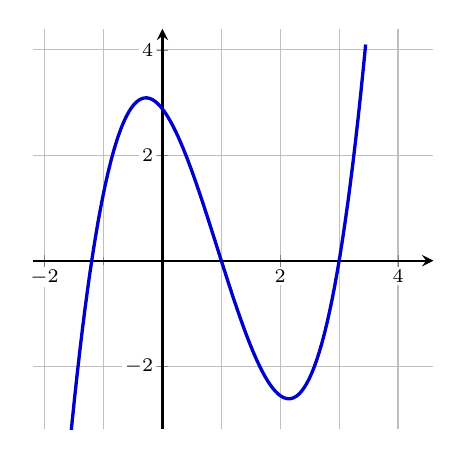
\begin{tikzpicture}
\begin{axis}[
  width=0.55\linewidth, height=0.55\linewidth,
  axis lines=middle, grid=both, minor tick num=1,
  xmin=-2.2, xmax=4.6, ymin=-3.2, ymax=4.4,
  xtick={-2,0,2,4}, ytick={-2,2,4},
  tick label style={font=\scriptsize}, ticklabel style={fill=white, inner sep=1pt},
  axis line style={thick},
]
\addplot[blue!80!black, very thick, samples=120, domain=-1.75:3.45]
  {0.8*(x+1.2)*(x-1)*(x-3)};
\end{axis}
\end{tikzpicture}
\end{center}
\figcaption{3.1}{Curve of a polynomial}

If a $<$ 0, the curve will have the shape:
\begin{center}
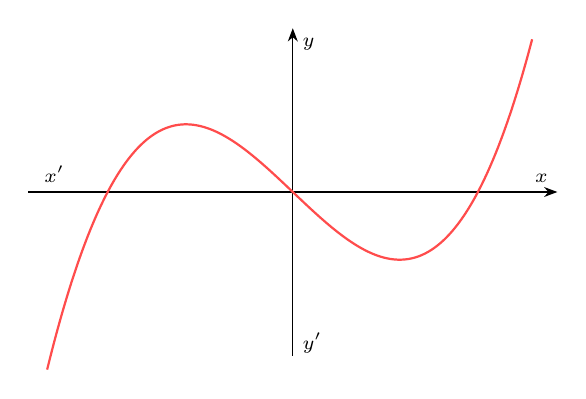
\begin{tikzpicture}[scale=0.8]
  \draw[-{Stealth}] (-4.2,0) -- (4.2,0) node[above left, font=\scriptsize] {$x$};
  \draw[-{Stealth}] (0,-2.6) -- (0,2.6) node[below right, font=\scriptsize] {$y$};
  \node[font=\scriptsize, above right] at (-4.1,0) {$x'$};
  \node[font=\scriptsize, right] at (0,-2.4) {$y'$};
  \draw[red!70, thick, samples=100, domain=-3.9:3.8, smooth]
    plot (\x, {0.11*\x*\x*\x - 0.95*\x});
\end{tikzpicture}
\end{center}
\figcaption{3.2}{Curve of a polynomial}

\textbf{Step 2:} Use the factor theorem or any known method to find the zeros of the
polynomial

\textbf{Step 3:} Find the y- intercept of the function by substituting x $=$ 0 into the
given polynomial function. (Note that this equates to the constant.)

\textbf{Step 4:} Find the intervals of the curve based on the zeros obtained

\textbf{Step 5:} Sketch the curve.

Individually, or in groups, let's use the steps for sketching polynomials to solve
the examples below.

\begin{example}{Example 3.6}
Sketch the curve $2x^3 + 3x^2 - 5x - 6$

\solution
\textbf{Step 1:} a is 2, which is greater than 0. Therefore, we know the shape that the
curve will take. The extremes will go from bottom left to top right.

\textbf{Step 2:} Using the factor theorem, the factors of the constant, - 6 are
$\pm 1, \pm 2, \pm 3, \pm 6$

Testing when x $=$ - 1, we have:

$2(-1)^3 + 3(-1)^2 - 5(-1) - 6 = -2 + 3 + 5 - 6 = 0$

Which means $(x + 1)$ is a factor.

We can use long division to find the other factors.
\[
\begin{array}{r@{\;}r}
 & 2x^2 + x - 6 \\ \cline{2-2}
x + 1\,\big) & 2x^3 + 3x^2 - 5x - 6 \\
 & \underline{-(2x^3 + 2x^2 + 0 + 0)} \\
 & x^2 - 5x - 6 \\
 & \underline{-(x^2 + x + 0)} \\
 & (-6x - 6) \\
 & \underline{-6x - 6}
\end{array}
\]
Factorising:

$2x^2 + x - 6$

$2x^2 + 4x - 3x - 6$

$2x(x + 2) - 3(x + 2)$

$(2x - 3)(x + 2)$

Factors are:

$(x + 1)(2x - 3)(x + 2)$

The zeros:

$(x + 1)(2x - 3)(x + 2) = 0$

$x = -1$, $x = -2$, $x = \frac{3}{2}$

\textbf{Step 3:} y intercept

When x $=$ 0

$2(0)^3 + 3(0)^2 - 5(0) - 6 = -6$

\textbf{Step 4}: finding the intervals using the zeros
\begin{center}
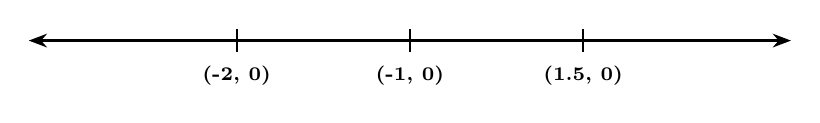
\begin{tikzpicture}[x=2.2cm]
  \draw[{Stealth}-{Stealth}, thick] (-0.7,0) -- (3.7,0);
  \foreach \x/\l in {0.5/{(-2, 0)}, 1.5/{(-1, 0)}, 2.5/{(1.5, 0)}} {
    \draw[thick] (\x,0.15) -- (\x,-0.15);
    \node[below, font=\scriptsize\bfseries] at (\x,-0.2) {\l};
  }
\end{tikzpicture}
\end{center}
The intervals are:
\begin{enumerate}
  \item $-2 < x$
  \item $-2 < x < -1$
  \item $-1 < x < 1.5$
  \item $x > 1.5$
\end{enumerate}
\booknote[S3-06]{the first interval is printed as $-2 < x$ (and $-1 < x$ in
Examples 3.7 and 3.8); the interval to the left of the first zero is $x < -2$
(respectively $x < -1$), as the table headings below show.}

Next is to determine the signs or test for the signs in each of the intervals obtained

\begin{center}
\small\renewcommand{\arraystretch}{1.2}
\begin{tabular}{|p{0.2\linewidth}|p{0.15\linewidth}|p{0.15\linewidth}|p{0.15\linewidth}|p{0.15\linewidth}|}
\hline
\textbf{Interval} & {\boldmath$-2 > x$} & {\boldmath$-2 < x < -1$} & {\boldmath$-1 < x < 1.5$} & {\boldmath$x > 1.5$} \\
\hline
Chosen values (you can choose any number within the interval)
& \centering\textbf{-3} & \centering\textbf{-1.5} & \centering\textbf{1} & \centering\textbf{2} \tabularnewline
\hline
$y$ value (substitute your chosen number into the given function)
& \centering $2(-3)^3 + 3(-3)^2 - 5(-3) - 6$ \par\medskip \textbf{= -18}
& \centering $2(-1.5)^3 + 3(-1.5)^2 - 5(-1.5) - 6$ \par\medskip \textbf{= 1.5}
& \centering $2(1)^3 + 3(1)^2 - 5(1) - 6$ \par\medskip \textbf{= -6}
& \centering $2(2)^3 + 3(2)^2 - 5(2) - 6$ \par\medskip \textbf{= 12} \tabularnewline
\hline
Sign & \centering Negative & \centering Positive & \centering Negative & \centering Positive \tabularnewline
\hline
Behaviour of curve & Below $x$ - axis & Above $x$ - axis & Below $x$ - axis & Above $x$ - axis \\
\hline
\end{tabular}
\end{center}

\textbf{Step 5:} sketch the curve
\begin{center}
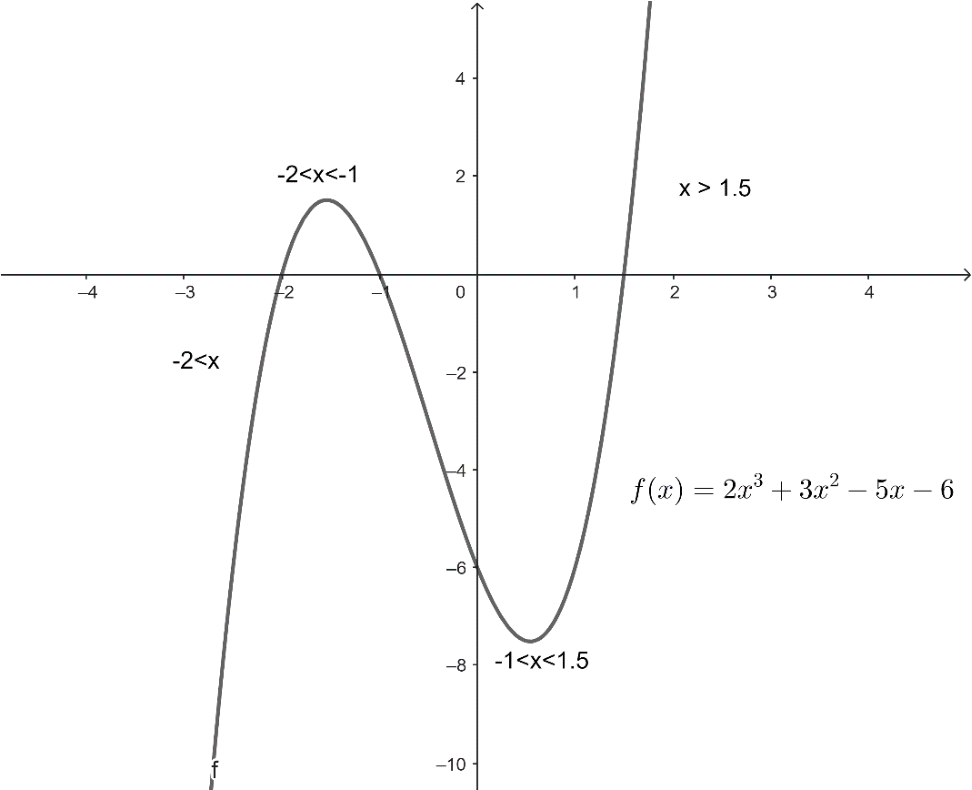
\includegraphics[width=0.75\linewidth]{figures/fig3-3.png}
\end{center}
\figcaption{3.3}{Curve of $2x^3 + 3x^2 - 5x - 6$}
\end{example}

\begin{example}{Example 3.7}
Sketch the curve $x^3 - 6x^2 + 5x + 12$

\solution
\textbf{Step 1:} a is 1 which is greater than 0. This means we know the shape the curve
will take.

\textbf{Step 2:} Using the factor theorem, the factors of the constant, 12 are
$\pm 1, \pm 2, \pm 3, \pm 4 \pm 6, \pm 12$

Testing when x $=$ - 1, we have:

$(-1)^3 - 6(-1)^2 + 5(-1) + 12$

$-1 - 6 - 5 + 12 = 0$

Which means $(x + 1)$ is a factor

We can use long division to find the other factors.
\[
\begin{array}{r@{\;}r}
 & x^2 - 7x + 12 \\ \cline{2-2}
x + 1\,\big) & x^3 - 6x^2 + 5x + 12 \\
 & \underline{-(x^3 + x^2 + 0 + 0)} \\
 & -7x^2 + 5x + 12 \\
 & (-7x^2 - 7x + 12) \\
 & 12x + 12 \\
 & \underline{-(12x + 12)} \\
 & 0
\end{array}
\]
\booknote[S3-07]{the line being subtracted is printed as $(-7x^2 - 7x + 12)$,
without the minus sign; it should be $-(-7x^2 - 7x + 0)$. The remainder line
$12x + 12$ and the quotient are correct.}

Factorising:

$x^2 - 7x + 12$

$x^2 - 4x - 3x + 12$

$x(x - 4) - 3(x - 4)$

$(x - 3)(x - 4)$

Factors are

$(x + 1)(x - 3)(x - 4)$

The zeros

$(x + 1)(x - 3)(x - 4) = 0$

$x = -1$, $x = 3$, $x = 4$

\textbf{Step 3:} $y$ intercept

At x $=$ 0

$(0)^3 - 6(0)^2 + 5(0) + 12 = 12$

\textbf{Step 4}: finding the intervals using the zeros
\begin{center}
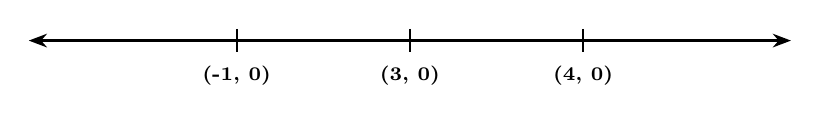
\begin{tikzpicture}[x=2.2cm]
  \draw[{Stealth}-{Stealth}, thick] (-0.7,0) -- (3.7,0);
  \foreach \x/\l in {0.5/{(-1, 0)}, 1.5/{(3, 0)}, 2.5/{(4, 0)}} {
    \draw[thick] (\x,0.15) -- (\x,-0.15);
    \node[below, font=\scriptsize\bfseries] at (\x,-0.2) {\l};
  }
\end{tikzpicture}
\end{center}
The interval are
\begin{enumerate}
  \item $-1 < x$
  \item $-1 < x < 3$
  \item $3 < x < 4$
  \item $x > 4$
\end{enumerate}
\booknote[S3-06]{see the note at Example 3.6: the first interval should be $x < -1$.}

Next is to determine the signs or test for the signs in each of the intervals obtained

\noindent\textbf{Table 3.1:} Test for signs in each of the intervals obtained
\begin{center}
\small\renewcommand{\arraystretch}{1.2}
\begin{tabular}{|p{0.2\linewidth}|p{0.15\linewidth}|p{0.15\linewidth}|p{0.15\linewidth}|p{0.15\linewidth}|}
\hline
\textbf{Interval} & {\boldmath$-2 > x$} & {\boldmath$-2 < x < -1$} & {\boldmath$-1 < x < 1.5$} & {\boldmath$x > 1.5$} \\
\hline
Chosen values (you can choose any number within the interval)
& \centering\textbf{-2} & \centering\textbf{1} & \centering\textbf{3.5} & \centering\textbf{5} \tabularnewline
\hline
y value (substitute your chosen number into the given function)
& \centering $(-2)^3 - 6(-2)^2 + 5(-2) + 12$ \par\medskip \textbf{= -30}
& \centering $(1)^3 - 6(1)^2 + 5(1) + 12$ \par\medskip \textbf{= 12}
& \centering $(3.5)^3 - 6(3.5)^2 + 5(3.5) + 12$ \par\medskip \textbf{= -1.125}
& \centering $2(5)^3 + 3(5)^2 - 5(5) - 6$ \par\medskip \textbf{= 294} \tabularnewline
\hline
Sign & \centering Negative & \centering Positive & \centering Negative & \centering Positive \tabularnewline
\hline
Behaviour of curve & Below x - axis & Above x - axis & Below x - axis & Above x - axis \\
\hline
\end{tabular}
\end{center}
\booknote[S3-08]{Table 3.1 repeats the interval headings of Example 3.6
($-2 > x$, $-2 < x < -1$, $-1 < x < 1.5$, $x > 1.5$) instead of $x < -1$,
$-1 < x < 3$, $3 < x < 4$, $x > 4$, and the last column evaluates the Example 3.6
polynomial $2x^3 + 3x^2 - 5x - 6$ at $x = 5$ (giving 294) instead of
$x^3 - 6x^2 + 5x + 12$, which gives 12. The sign, Positive, is unchanged.}

\begin{center}
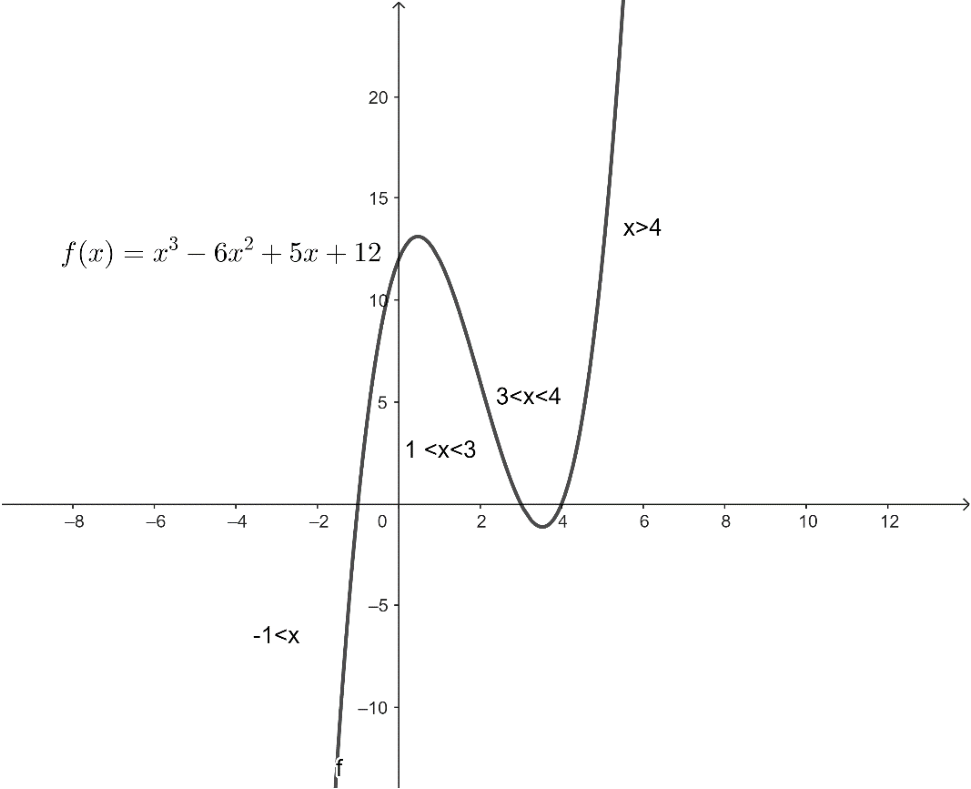
\includegraphics[width=0.75\linewidth]{figures/fig3-4.png}
\end{center}
\figcaption{3.4}{Curve of $x^3 - 6x^2 + 5x + 12$}
\end{example}

\begin{example}{Example 3.8}
Sketch the curve $-x^3 + 4x^2 - x - 6$

\solution
\textbf{Step 1:} a is -1 which is less than 0. This means that the extremes of the graph
go from top left to bottom right.

\textbf{Step 2:} Using the factor theorem, the factors of the constant, -6 are
$\pm 1, \pm 2, \pm 3, \pm 6$

Testing when x $=$ 2, we have:

$-(2)^3 + 4(2)^2 - 2 - 6 = -8 + 16 - 2 - 6 = 0$

Which means $(x - 2)$ is a factor.

We can use long division to find the other factors.
\[
\begin{array}{r@{\;}r}
 & -x^2 + 2x + 3 \\ \cline{2-2}
x - 2\,\big) & -x^3 + 4x^2 - x - 6 \\
 & \underline{-(-x^3 + 2x^2 + 0 + 0)} \\
 & 2x^2 - x - 6 \\
 & -(2x^2 - 4x - 6) \\
 & 3x - 6 \\
 & \underline{-(3x - 6)} \\
 & 0
\end{array}
\]
\booknote[S3-09]{the second subtraction is printed as $-(2x^2 - 4x - 6)$; the
line being subtracted is $2x(x - 2) = 2x^2 - 4x + 0$. The remainder $3x - 6$
and the quotient are correct.}

Factorising:

$-x^2 + 2x + 3$

$-x^2 + 3x - x + 3$

$-x(x - 3) - 1(x - 3)$

$(-x - 1)(x - 3)$

Factors are

$(x - 2)(x - 3)(-x - 1)$

The zeros

$(x - 2)(x - 3)(-x - 1) = 0$

$x = -1$, $x = 3$, $x = 2$

\textbf{Step 3:} y intercept:

When x $=$ 0

$-(0)^3 + 4(0)^2 - (0) - 6 = -6$

\textbf{Step 4}: finding the intervals using the zeros
\begin{center}
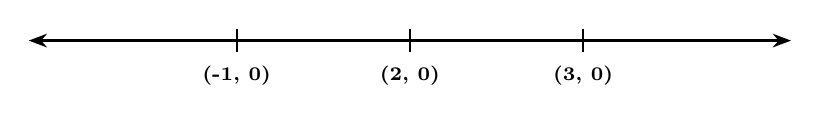
\begin{tikzpicture}[x=2.2cm]
  \draw[{Stealth}-{Stealth}, thick] (-0.7,0) -- (3.7,0);
  \foreach \x/\l in {0.5/{(-1, 0)}, 1.5/{(2, 0)}, 2.5/{(3, 0)}} {
    \draw[thick] (\x,0.15) -- (\x,-0.15);
    \node[below, font=\scriptsize\bfseries] at (\x,-0.2) {\l};
  }
\end{tikzpicture}
\end{center}
The intervals are
\begin{enumerate}
  \item $-1 < x$
  \item $-1 < x < 2$
  \item $2 < x < 3$
  \item $x > 3$
\end{enumerate}
\booknote[S3-06]{see the note at Example 3.6: the first interval should be $x < -1$.}

Next is to determine the signs or test for the signs in each of the intervals obtained

\noindent\textbf{Table 3.2:} Test for signs in each of the intervals obtained
\begin{center}
\small\renewcommand{\arraystretch}{1.2}
\begin{tabular}{|p{0.2\linewidth}|p{0.15\linewidth}|p{0.15\linewidth}|p{0.15\linewidth}|p{0.15\linewidth}|}
\hline
\textbf{Interval} & {\boldmath$-1 > x$} & {\boldmath$-1 < x < 2$} & {\boldmath$2 < x < 3$} & {\boldmath$x > 3$} \\
\hline
Chosen values (you can choose any number within the interval)
& \centering\textbf{-3} & \centering\textbf{1} & \centering\textbf{2.5} & \centering\textbf{4} \tabularnewline
\hline
y value (substitute your chosen number into the given function)
& \centering $-(-3)^3 + 4(-3)^2 - (-3) - 6$ \par\medskip \textbf{= 60}
& \centering $-(1)^3 + 4(1)^2 - (1) - 6$ \par\medskip \textbf{= -4}
& \centering $-(2.5)^3 + 4(2.5)^2 - (2.5) - 6$ \par\medskip \textbf{= 0.875}
& \centering $-(4)^3 + 4(4)^2 - (4) - 6$ \par\medskip \textbf{= -10} \tabularnewline
\hline
Sign & \centering Positive & \centering Negative & \centering Positive & \centering Negative \tabularnewline
\hline
Behaviour of curve & Above $x$ - axis & Below $x$ - axis & Above $x$ - axis & Below $x$ - axis \\
\hline
\end{tabular}
\end{center}

\begin{center}
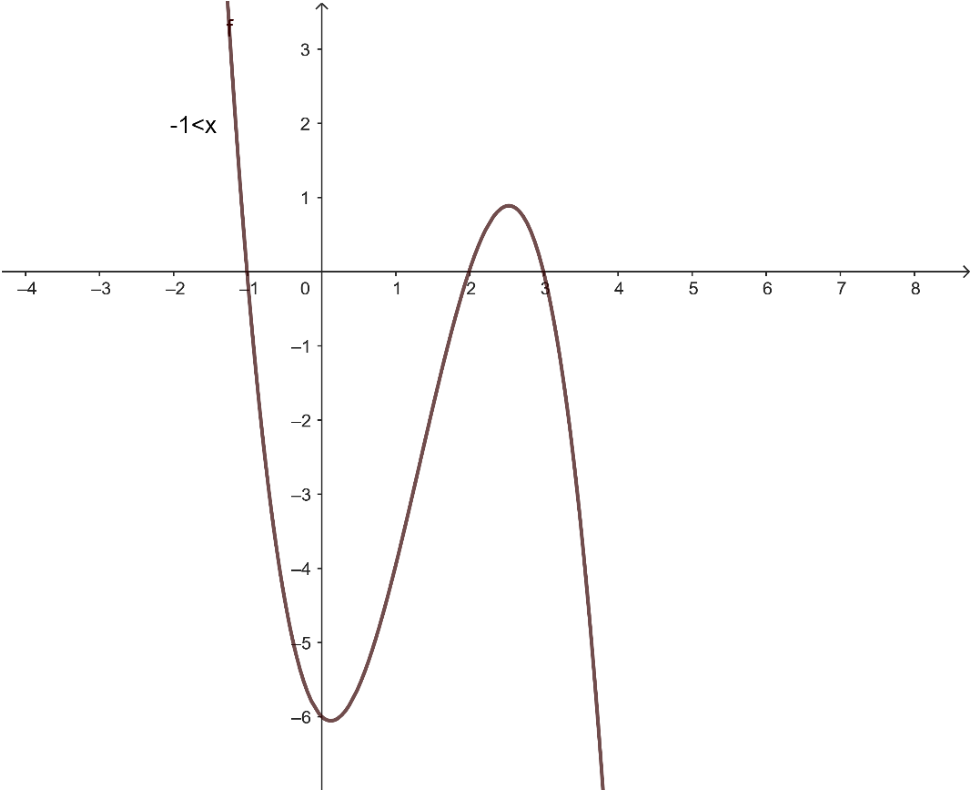
\includegraphics[width=0.75\linewidth]{figures/fig3-5.png}
\end{center}
\figcaption{3.5}{\textit{Curve of} $-x^3 + 4x^2 - x - 6$}
\end{example}

What polynomial function is represented in the graph below?
\begin{enumerate}
  \item[a.] How many factors does it have?
  \item[b.] Share your answers with the class.
\end{enumerate}
\begin{center}
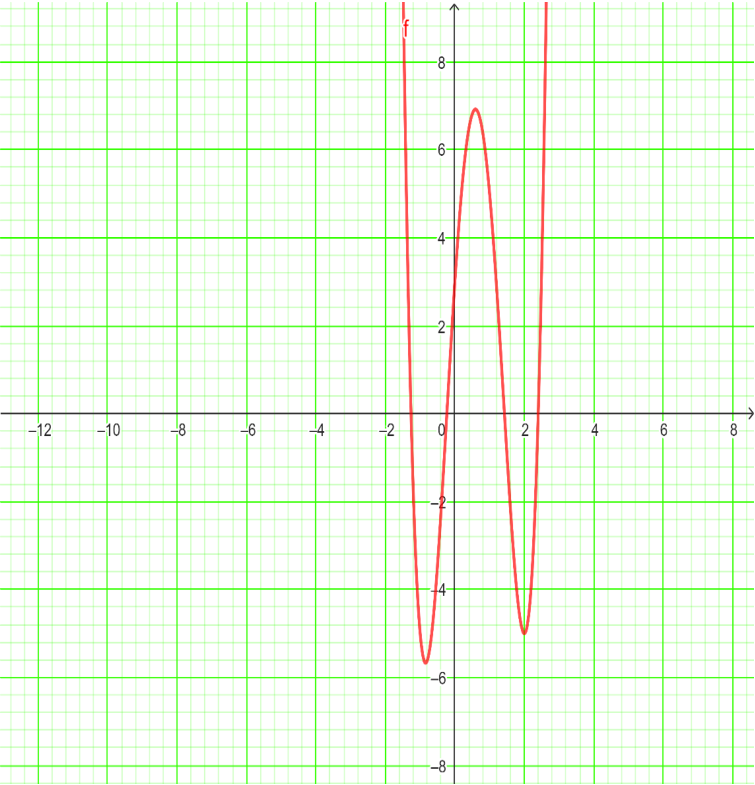
\includegraphics[width=0.6\linewidth]{figures/fig3-6.png}
\end{center}
\figcaption{3.6}{Graph of a polynomial function}

Remember that it is an important skill to be able to sketch graphs by hand.
However, when appropriate technology is there to assist. For example, you can
use apps or web-based programs such as GeoGebra, Demos, PhET Simulations
and Geometer's Sketch Pad.

% Book pp. 111-116 (PDF pp. 112-117)
\section{Applying Descartes' Rule of Signs Theorem}

There is another way that can be used to determine how many positive and negative
real zeros a polynomial function might have. To do this, first write the polynomial
in descending order (from the highest degree to the lowest) if it is not already. We
use \textbf{Descartes' Rule of Signs}. This rule helps you see how the number of times
the signs change in the polynomial is related to the number of positive real zeros.

For example, if you look at the polynomial function below, you will notice it has
one sign change, which gives you information about its positive zeros.

Let us go through an example using Descartes' Rule of Signs to determine the
possible number of positive and negative real zeros.

\begin{example}{Example 3.9}
Consider the polynomial:

$f(x) = 3x^3 - 2x^2 + 4x - 5$

\solution
\textbf{Step 1:} \textit{Identify Sign Changes for Positive Real Zeros}
\begin{enumerate}
  \item Write the polynomial in descending order:
  \item $f(x) = 3x^3 - 2x^2 + 4x + 5$
  \booknote[S3-10]{the polynomial is $3x^3 - 2x^2 + 4x - 5$, as in the question
  and in the coefficient list that follows; the ``$+ 5$'' is a misprint.}

  Look at the coefficients:

  3 (positive)

  --2 (negative)

  4 (positive)

  $-5$ (negative)
  \item Determine the sign changes:

  From 3 to -2 (1 change)

  From $-2$ to 4 (2 changes)

  From 4 to $-5$ (3 changes)

  Total sign changes for positive zeros $=$ 3. This means there could be 3,
  (3 -- 2 $=$ 1) positive real zeros. Note, the number of possible roots is found by
  subtracting 2 each time until we would get a negative number.
\end{enumerate}
\textbf{Step 2:} \textit{Identify Sign Changes for Negative Real Zeros}
\begin{quote}
Now, let's find the negative real zeros by evaluating f($-x$):

$f(-x) = 3(-x)^3 - 2(-x)^2 + 4(-x) - 5$

$f(-x) = -3x^3 - 2x^2 - 4x - 5$
\end{quote}
\textbf{Step 3:} \textit{Look at the Signs of f($-x$)}
\begin{quote}
The coefficients are:

$-3$ (negative)

$-2$ (negative)

$-4$ (negative)

$-5$ (negative)
\end{quote}
\textbf{Step 4:} \textit{Determine Sign Changes for Negative Real Zeros}
\begin{quote}
There are \textbf{no sign changes} in f($-$x)
\end{quote}
Total sign changes for negative zeros $=$ 0. This means there are no negative real
roots or zeros.
\end{example}

This example illustrates how to use Descartes' Rule of Signs to analyse a polynomial
and determine the possible numbers of positive and negative real zeros.

Let us solve more examples.

\begin{example}{Example 3.10}
Use Descartes' Rule of Signs to determine how many possible positive and
negative real zeros of the following:
\begin{enumerate}
  \item[a.] $g(x) = 2x^4 - 11x^3 + 4x^2 - 8x - 40$
  \item[b.] $g(x) = 9x^3 - 10x^2 + 5x + 3$
  \item[c.] f$(x) = -x^5 + 3x^4 - 5x^3 - 12x^2 + 6x + 4$
\end{enumerate}

\solution
\begin{enumerate}
  \item[a.] $g(x) = 2x^4 - 11x^3 + 4x^2 - 8x - 40$
\end{enumerate}
\textbf{Step 1:} \textit{Identify Sign Changes for Positive Real Zeros}
\begin{quote}
Write the polynomial in descending order:

$g(x) = 2x^4 - 11x^3 + 4x^2 - 8x - 40$

Look at the coefficients:

2 (positive)

--11 (negative)

4 (positive)

$-8$ (negative)

$-40$ (negative)

Look at the coefficients:

Determine the sign changes:

From 2 to -11 (1 change)

From $-11$ to 4 (2 changes)

From 4 to $-8$ (3 changes)

From -8 to $-40$ (no change)

Total sign changes for positive zeros $=$ 3. This means there could be 3 or 1
positive real zeros.
\end{quote}
\textbf{Step 2:} \textit{Identify Sign Changes for Negative Real Zeros}
\begin{quote}
Now, let's find the negative real zeros by evaluating f($-$x):

$g(x) = 2(-x)^4 - 11(-x)^3 + 4(-x)^2 - 8(-x) - 40$

$g(x) = 2x^4 + 11x^3 + 4x^2 + 8x - 40$
\end{quote}
\textbf{Step 3:} \textit{Look at the Signs of f($-x$)}
\begin{quote}
The coefficients are:

2 (positive)

11 (positive)

4 (positive)

8 (positive)

$-40$ (negative)
\end{quote}
\textbf{Step 4:} \textit{Determine Sign Changes for Negative Real Zeros}
\begin{quote}
Determine the sign changes:

From 2 to 11 (no change)

From 11 to 4 (no changes)

From 4 to 8 (no changes)

From 8 to $-40$ (1 change)

Total sign changes for negative zeros $=$ 1. This means there is 1 negative
real zero.
\end{quote}
\begin{enumerate}
  \item[b.] $g(x) = 9x^3 - 10x^2 + 5x + 3$
\end{enumerate}
\textbf{Step 1:} \textit{Identify Sign Changes for Positive Real Zeros}
\begin{quote}
Write the polynomial in descending order: $g(x) = 9x^3 - 10x^2 + 5x + 3$.

Look at the coefficients:

9 (positive)

$-10$ (negative)

5 (positive)

3 (negative)
\booknote[S3-11]{3 is positive; the sign changes counted below (2) are right.}

Determine the sign changes:

From 9 to -10 (1 change)

From $-10$ to 5 (2 changes)

From 5 to 3 (no change)

Total sign changes for positive zeros $=$ 2. This means there could be 2 or 0.
\end{quote}
\textbf{Step 2:} \textit{Identify Sign Changes for Negative Real Zeros}
\begin{quote}
Now, let's find the negative real zeros by evaluating g($-$x):

$g(x) = 9(-x)^3 - 10(-x)^2 + 5(-x) + 3$

$g(x) = -9x^3 - 10x^2 - 5x + 3$
\end{quote}
\textbf{Step 3:} \textit{Look at the Signs of f($-x$)}
\begin{quote}
The coefficients are:

$-9$ (negative)

$-10$ (negative)

$-5$ (negative)

3 (positive)
\end{quote}
\textbf{Step 4:} \textit{Determine Sign Changes for Negative Real Zeros}
\begin{quote}
Determine the sign changes:

From -9 to -10 (no change)

From -10 to -5 (no changes)

From -5 to 3 (1 change)

Total sign changes for negative zeros $=$ 1. This means there is 1 negative
real zero.
\end{quote}
\begin{enumerate}
  \item[c.] f$(x) = -x^5 + 3x^4 - 5x^3 - 12x^2 + 6x + 4$
\end{enumerate}
\textbf{Step 1:} \textit{Identify Sign Changes for Positive Real Zeros}
\begin{quote}
Write the polynomial in descending order:

f$(x) = -x^5 + 3x^4 - 5x^3 - 12x^2 + 6x + 4$

Look at the coefficients:

$-1$ (negative)

3 (positive)

$-5$ (negative)

$-12$ (negative)

6 (positive)

4 (positive)

\textit{Determine the sign changes:}

From $-1$ to 3 (1 change)

From 3 to $-5$ (2 changes)

\textbf{From $-5$ to $-12$ (no changes)}

From $-12$ to 6 (3 changes)

From 6 to 4 (no change)

Total sign changes for positive zeros $=$ 3. This means there could be 3 or 1
positive real zeros.
\end{quote}
\textbf{Step 2:} \textit{Identify Sign Changes for Negative Real Zeros}
\begin{quote}
Now, let's find the negative real zeros by evaluating f($-$x):

f$(x) = -(-x)^5 + 3(-x)^4 - 5(-x)^3 - 12(-x)^2 + 6(-x) + 4$

f$(x) = x^5 + 3x^4 + 5x^3 - 12x^2 - 6x + 4$
\end{quote}
\textbf{Step 3:} Look at the Signs of f($-$x)
\begin{quote}
The coefficients are:

1 (positive)

3 (positive)

5 (positive)

--12 (negative)

--6 (negative)

4 (positive)
\end{quote}
\textbf{Step 4:} \textit{Determine Sign Changes for Negative Real Zeros}
\begin{quote}
Determine the sign changes:

From 1 to 3 (no change)

From 3 to 5 (no changes)

From 5 to $-12$ (2 changes)

From $-2$ to $-6$ no changes)
\booknote[S3-12]{``From $-2$'' should read ``From $-12$''; and the count of changes
in the line above (2) should be 1, the line below 2, giving the printed total of 2.}

From $-6$ to 4 (3 change)

Total sign changes for negative zeros $=$ 2. This means there is 2 or 0 negative
real zeros.
\end{quote}
\end{example}

% Book pp. 116-122 (PDF pp. 117-123)
\section{Applying the Fundamental Theorem of Algebra}

The \textbf{Fundamental Theorem of Algebra} tells us something very important about
polynomial functions. It says: `Every polynomial function of degree $n$ (where $n >
0$) has at least one complex zero.'

This might sound complicated at first, but here is what it means:
\begin{enumerate}
  \item The degree of a polynomial is the highest power of $x$ in the expression.
  \item For example, $x^3 - 2x^2 + 4x - 8$ has a degree of 3.
  \item Complex numbers include real numbers and imaginary numbers (numbers
  with $i$, where $i = \sqrt{-1}$)
  \item In factorising the polynomial, each root c$_i$ corresponds to a linear factor of
  the form $(x - c_i)$. This means we can write the polynomial as f(x) $= a\,(x -
  c_1)\,(x - c_2) \cdots (x - c_n)$.

  The, $a$ is a non-zero number that affects how the polynomial behaves, and
  $c_1, c_2, \ldots, c_n$, are the roots, or zeros.
\end{enumerate}
Let us go through these examples to show how it works.

\begin{example}{Example 3.11}
Factorise the polynomial f$(x) = 3x^5 - 48x$ completely and find all its zeros.

State the multiplicity of each zero.

\solution
f$(x) = 3x^5 - 48x$

Factorising:

$3x(x^4 - 16)$

$3x[(x^2)^2 - 4^2]$

$3x[(x^2 + 4)(x^2 - 4)]$

$3x[x^2 - (-4)(x^2 - 4)]$

$3x[(x + 2i)(x - 2i)(x + 2)(x - 2)]$

To find the zeros, equate the factors to zero:

$3x[(x + 2i)(x - 2i)(x + 2)(x - 2)] = 0$

$3x = 0$, $x = 0$

$x + 2i = 0$, $x = -2i$

$x - 2i = 0$, $x = 2i$

$x + 2 = 0$, $x = -2$

$x - 2 = 0$, $x = 2$

Therefore, the zeros of f($x$) are 0, 2, -- 2, 2$i$ and -- 2$i$. Since each factor occurs
only once, all the zeros are of multiplicity 1 and the total number of zeros is five.
\end{example}

\begin{example}{Example 3.12}
Factorise the polynomial f$(x) = x^4 - 625$ completely and find all its zeros.

State the multiplicity of each zero.

\solution
f$(x) = x^4 - 625$

Factorising:

$(x^4 - 625)$

$[(x^2)^2 - 25^2]$

$[(x^2 + 25)(x^2 - 25)]$

$3x[x^2 - (-25)(x^2 - 25)]$
\booknote[S3-13]{the ``$3x$'' is carried over from Example 3.11; there is no such
factor here.}

$[(x + 5i)(x - 5i)(x + 5)(x - 5)]$

To find the zeros, equate the factors to zero:

$[(x + 5i)(x - 5i)(x + 5)(x - 5)] = 0$

$x + 5i = 0$, $x = -5i$

$x - 5i = 0$, $x = 5i$

$x + 5 = 0$, $x = -5$

$x - 5 = 0$, $x = 5$

Therefore, the zeros of f($x$) are 5, -- 5, 5$i$ and -- 5$i$. Since each factor occurs
only once, all the zeros are of multiplicity 1 and the total number of zeros is four.
\end{example}

\begin{example}{Example 3.13}
Factorise the polynomial f$(x) = 15x^4 + 8x^2 + 1$ completely and find all its zeros.

State the multiplicity of each zero.

\solution
f$(x) = 15x^4 + 8x^2 + 1$

in this scenario, we can represent $x^2$ by any other letter, for example, u

$f(x) = 15(x^2)^2 + 8x^2 + 1$

$f(x) = 15(u)^2 + 8u + 1$

$15u^2 + 8u + 1$

Factorising:

$15u^2 + 5u + 3u + 1$

$5u(3u + 1) + (3u + 1)$

$(5u + 1)(3u + 1)$

Substituting $x^2$ back,

$(5x^2 + 1)(3x^2 + 1)$

To find the zeros, equate the factors to zero:

$(5x^2 + 1)(3x^2 + 1) = 0$

$5x^2 + 1 = 0$ or $3x^2 + 1 = 0$

For $5x^2 + 1 = 0$

$5x^2 = -1$

$x^2 = -\frac{1}{5}$

$x = \pm\sqrt{-\frac{1}{5}}$

$x = -\sqrt{-\frac{1}{5}}$ or $x = \sqrt{-\frac{1}{5}}$

For $x = -\sqrt{-\frac{1}{5}}$

$x = -\sqrt{\frac{1}{5}} \times \sqrt{-1}$

$x = -i\sqrt{\frac{1}{5}}$

$x = -\frac{\sqrt{5}}{5}\,i$

For $x = \sqrt{-\frac{1}{5}}$

$x = \sqrt{\frac{1}{5}} \times \sqrt{-1}$

$x = i\sqrt{\frac{1}{5}}$

$x = \frac{\sqrt{5}}{5}\,i$

For $3x^2 + 1 = 0$

$3x^2 = -1$

$x^2 = -\frac{1}{3}$

$x = \pm\sqrt{-\frac{1}{3}}$

$x = -\sqrt{-\frac{1}{3}}$ or $x = \sqrt{-\frac{1}{3}}$

For $x = -\sqrt{-\frac{1}{3}}$

$x = -\sqrt{\frac{1}{3}} \times \sqrt{-1}$

$x = -i\sqrt{\frac{1}{3}}$

$x = -\frac{\sqrt{3}}{3}\,i$

For $x = \sqrt{-\frac{1}{3}}$

$x = \sqrt{\frac{1}{3}} \times \sqrt{-1}$

$x = i\sqrt{\frac{1}{3}}$

$x = \frac{\sqrt{3}}{3}\,i$

Therefore, the zeros of $f(x)$ $\frac{\sqrt{3}}{3}\,i, -\frac{\sqrt{3}}{3}\,i,
-\frac{\sqrt{5}}{5}\,i, \frac{\sqrt{5}}{5}\,i$. Since each factor occurs only once, all
the zeros are of multiplicity 1 and the total number of zeros is four.
\end{example}

\begin{example}{Example 3.14}
Factorise the polynomial f$(x) = x^4 - 4x^2 - 21$ completely and find all its zeros.

State the multiplicity of each zero.

\solution
f$(x) = x^4 - 4x^2 - 21$

in this scenario, we can represent $x^2$ by u

$f(x) = (x^2)^2 - 4x^2 - 21$

$f(x) = (u)^2 - 4u - 21$

$u^2 - 4u - 21$

Factorising:

$u^2 - 7u + 3u - 21$

$u(u - 7) + 3(u - 7)$

$(u + 3)(u - 7)$

Substituting $x^2$ back,

$(x^2 + 3)(x^2 - 7)$

To find the zeros, equate the factors to zero:

$(x^2 + 3)(x^2 - 7) = 0$

$x^2 + 3 = 0$ or $x^2 - 7 = 0$

For $x^2 + 3 = 0$

$x^2 = -3$

$x^2 = -3$

$x = \pm\sqrt{-3}$

$x = -\sqrt{-3}$ or $x = \sqrt{-3}$

For $x = -\sqrt{-3}$

$\sqrt{-3} = -\sqrt{3} \times \sqrt{-1}$

$x = -\sqrt{3} \times \sqrt{-1}$

$x = -i\sqrt{3}$

For $x = \sqrt{-3}$

$x = \sqrt{3} \times \sqrt{-1}$

$x = i\sqrt{3}$

For $x^2 - 7$

$x^2 = 7$

$x^2 = 7$

$x = \pm\sqrt{7}$

$x = -\sqrt{7}$ or $x = \sqrt{7}$

For $x = -\sqrt{7}$

$x = -\sqrt{7}$

For $x = \sqrt{7}$

$x = \sqrt{7}$

$x = \sqrt{7}$

Therefore, the zeros of $f(x)$ are $x = i\sqrt{3}$, $x = -i\sqrt{3}$, $x = -\sqrt{7}$,
$x = \sqrt{7}$. Since each factor occurs only once, all the zeros are of multiplicity
1 and the total number of zeros is four.
\end{example}

Note: Multiplicity refers to the number of times a particular zero (or root) appears
in the factorisation of a polynomial. It indicates how many times a specific value
$x = r$ is a solution to the polynomial equation P($x$) $=$ 0.

\noindent\textit{\color{blue}Key Points about Multiplicity:}
\begin{enumerate}
  \item Simple Roots: If a root appears once, it has a multiplicity of 1. For example,
  in the polynomial $(x - 2)$, the root $x = 2$ has multiplicity 1.
  \item Repeated Roots: If a root appears more than once, it has a higher multiplicity.
  For example, in the polynomial $(x - 2)^2$, the root $x = 2$ has a multiplicity of
  2.
  \item Multiplicity and Behaviour: This can be even or odd.
\end{enumerate}
\textit{Odd Multiplicity}: If a root has an odd multiplicity, the graph of the polynomial
crosses the $x$ - axis at that root.

\textit{Even Multiplicity}: If a root has an even multiplicity, the graph of the polynomial
touches the x-axis at that root but does not cross it.

For instance, for the polynomial P(x) $= (x - 1)\,(x - 1)\,(x + 2)$:

The root $x = 1$ has a multiplicity of 2 (it appears twice), so the graph just touches
the x-axis at x $=$ 1 and does not cross it.

The root $x = -2$ has a multiplicity of 1 (it appears once), so the graph crosses the
x-axis at x $=$ -2.

% Book pp. 122-125 (PDF pp. 123-126)
\section{Complex Conjugates Theorem}

\textbf{Complex Numbers}: A complex number is expressed in the form $a + bi$, where a
and b are real numbers, and $i$ is the imaginary unit defined as $i^2 = -1$, or
$i = \sqrt{-1}$

\textbf{Roots of Polynomials}: When dealing with polynomial equations, the Fundamental
Theorem of Algebra states that every non-constant polynomial has at least one
complex root. This means that if a polynomial has real coefficients, any non-real
roots must occur in conjugate pairs.

If $a + bi$ (where b $\ne$ 0) is a root of a polynomial, then its conjugate $a - bi$ is
also a root.

\textbf{Example}: For a polynomial like $x^2 + 4$:

The roots can be found by rearranging to $x^2 = -4$.

Taking the square root gives $x = \pm 2i$

Here, $2i$ and $-2i$ are complex roots that come in conjugate pairs.

\textbf{Note that:}

\textbf{Complex roots} always come in \textbf{conjugate pairs}.

If $a + bi$ is a root of a polynomial, then $a - bi$ is also a root.

This property helps us find all the roots of polynomials, ensuring we account for
both real and complex solutions.

The \textbf{Complex Conjugate Theorem} states that if a polynomial has a complex
root, its conjugate must also be a root. This is an important concept in algebra that
helps us understand the nature of polynomial equations and their solutions.

Let us go through the following examples to explore how to use the \textbf{Complex
conjugate theorem.}

For example, if we are given one complex factor of a polynomial, we know
another factor must be the complex conjugate. This gives us two factors. We can
then form a quadratic equation and use algebraic division to find another factor.
Or we may be given two real factors, for example, $x = 2$ and $x = -3$. This means
that $x - 2 = 0$ or $x + 3 = 0$

$\therefore (x - 2)(x + 3) = 0$

$x^2 + 3x - 2x - 6 = 0$

$x^2 + x - 6 = 0$

\begin{example}{Example 3.15}
Find all the roots of $f(x) = x^3 + 8x^2 + 21x + 20$ if one root is -2 $-$ $i$.

\solution
$f(x) = x^3 + 8x^2 + 21x + 20$

Since the factor given $(-2 - i)$ is complex in nature, we need the conjugate as
well: $-2 + i$

$[x - (-2 - i)][(x - (-2 + i)]$

$[x + 2 + i][x + 2 - i]$

$(x + 2)^2 - (i)^2$

$x^2 + 4x + 4 - i^2$

NB: $-i^2 = 1$

$x^2 + 4x + 4 - (-1)$

$x^2 + 4x + 5$

We can use long division to find the other factors:
\[
\begin{array}{r@{\;}r}
 & x + 4 \\ \cline{2-2}
x^2 + 4x + 5\,\big) & x^3 + 8x^2 + 21x + 20 \\
 & \underline{-(x^3 + 4x^2 + 5x + 20)} \\
 & 4x^2 + 16x + 20 \\
 & \underline{-(4x^2 + 16x + 20)} \\
 & 0
\end{array}
\]
$x + 4 = 0$

$x = -4$

Therefore, the roots of $(x)$ are $-4$, $-2 + i$ and $-2$ -- $i$
\end{example}

\begin{example}{Example 3.16}
Find all the roots of $f(x) = 2x^3 - 13x^2 + 26x - 10$ if one root is $3 + i$.

\solution
$f(x) = 2x^3 - 13x^2 + 26x - 10$

Since the factor given $3 + i$. is complex in nature, we need the conjugate as well:
$3 - i$

$[x - (3 + i)][(x - (3 - i)]$

$[x - 3 - i][x - 3 + i]$

$(x - 3)^2 - (i)^2$

$x^2 - 6x + 9 - i^2$

NB: $-i^2 = -1$
\booknote[S3-14]{$-i^2 = 1$, as Example 3.15 states; the next line correctly
subtracts $(-1)$.}

$x^2 - 6x + 9 - (-1)$

$x^2 - 6x + 10$

We can use long division to find the other factor.
\[
\begin{array}{r@{\;}r}
 & 2x - 1 \\ \cline{2-2}
x^2 - 6x + 10\,\big) & 2x^3 - 13x^2 + 26x - 10 \\
 & \underline{-(2x^3 - 12x^2 + 20x + 0)} \\
 & -x^2 + 6x - 10 \\
 & \underline{-(-x^2 + 6x - 10)} \\
 & 0
\end{array}
\]
$2x - 1 = 0$

$x = \frac{1}{2}$

Therefore, the roots of $(x)$ are $= \frac{1}{2}$, $3 + i$ and $3$ -- $i$
\end{example}

% Book pp. 125-128 (PDF pp. 126-129)
\section{Linear and Quadratic Factor Theorems}

The linear quadratic factor theorem is another method which can be used to solve
polynomial functions. This is when we break polynomial functions into linear and
quadratic factors to make solving it simpler.

For example, to use the linear and quadratic factor approach to find the factors of
$x^4 - 9x^2 + 14$, we:

\textbf{Step 1}: Let $x^2 = u$

\textbf{Step 2}: Using this substitution it means $x^4 - 9x^2 + 14 = (u)^2 - 9(u) + 14$

\textbf{Step 3}: Factorise $u^2 - 9u + 14$:

$u^2 - 7u - 2u + 14$

$u(u - 7) - 2(u - 7)$

$(u - 2)(u - 7)$

\textbf{Step 4}: Substitute $x^2$ back in for $u$:

$(x^2 - 2)(x^2 - 7)$

$x^2 - 2 = 0$ and $x^2 - 7 = 0$

For $x^2 - 2 = 0$

$x^2 = 2$

$x = \pm\sqrt{2}$

$x = -\sqrt{2}$ or $x = \sqrt{2}$

$x + \sqrt{2}$ and $x - \sqrt{2}$ are factors

For $x^2 - 7 = 0$

$x^2 = 7$

$x = \pm\sqrt{7}$

$x = -\sqrt{7}$ or $x = \sqrt{7}$

$x + \sqrt{7}$ and $x - \sqrt{7}$ are factors

Hence the factors are $+\sqrt{2}$, $x - \sqrt{2}$, $x + \sqrt{7}$ and $x - \sqrt{7}$

\begin{example}{Example 3.17}
Given $f(x) = x^4 - 1$, find all the factors using the linear quadratic factor approach.

\solution
Let $u = x^2$

$f(x) = (x^2)^2 - 1$

$(u)^2 - 1$

$u^2 - 1$

Factorising:

$(u - 1)(u + 1)$

Substituting $x^2$ back in:

$(x^2 - 1)(x^2 + 1)$

$(x^2 - 1)(x^2 + 1) = 0$

$x^2 - 1 = 0$ or $x^2 + 1 = 0$

For $x^2 - 1 = 0$

$x^2 = \pm 1$

$x = 1$ or $x = -1$

For $(x^2 + 1)$

$x^2 + 1 = 0$

$x^2 = -1$

$x = \pm\sqrt{-1}$

\textbf{NB:} $\sqrt{-1} = \boldsymbol{i}$

$x = \pm i$

$x = -i$ or $x = i$

Hence the factors are $(x + 1)$, $(x - 1)$, $(x - i)(x + i)$
\end{example}

\begin{example}{Example 3.18}
Given $f(x) = 2x^4 + x^2 - 10$, find all the factors using the linear quadratic factor
approach

\solution
Let $u = x^2$

$f(x) = 2(x^2)^2 + u - 10$

$2(u)^2 + u - 10$

$2u^2 + u - 10$

Factorising:

$2u^2 - 4u + 5u - 10$

$2u(u - 2) + 5(u - 2)$

$(2u + 5)(u - 2)$

Substituting:

$u = x^2$

$(2x^2 + 5)(x^2 - 2)$

$(2x^2 + 5)(x^2 - 2) = 0$

$2x^2 + 5 = 0$ or $x^2 - 2 = 0$

For $2x^2 + 5 = 0$

$x^2 = -\frac{5}{2}$

$x = \pm\sqrt{-\frac{5}{2}}$

$x = \frac{5}{2}\,i$ or $x = -\frac{5}{2}\,i$
\booknote[S3-15]{$\sqrt{-\frac{5}{2}} = \sqrt{\frac{5}{2}}\,i = \frac{\sqrt{10}}{2}\,i$,
not $\frac{5}{2}\,i$; the two complex factors in the last line inherit the slip.}

For $(x^2 - 2)$

$x^2 - 2 = 0$

$x^2 = 2$

$x = \pm\sqrt{2}$

$x = -\sqrt{2}$ or $x = \sqrt{2}$

Hence the factors are $\left(x + \frac{5}{2}\,i\right)\left(x - \frac{5}{2}\,i\right)
\left(x - \sqrt{2}\right)\left(x + \sqrt{2}\right)$
\end{example}

We can use what we have learned to help in determining the maximum or minimum
profit or productivity in the real world.

In small groups, or individually, discuss how the following problem can be solved.

\begin{example}{Example 3.19}
A water production company made sales of $x$ bags of water and the profit was
given by $2x^2 + 7x - 15$ where $0 \le x \le 10$.

Help the company determine their maximum profit and loss.

\solution
Since the range was given \textbf{(}$0 \le x \le 10$), we do our calculation within
this range.

Evaluating the function in the given interval, we obtain:
\begin{center}
\renewcommand{\arraystretch}{1.3}
\begin{tabular}{|l|c|c|c|c|c|c|c|c|c|c|c|}
\hline
x & 0 & 1 & 2 & 3 & 4 & 5 & 6 & 7 & 8 & 9 & 10 \\
\hline
$2x^2 + 7x - 15$ & -15 & -6 & 7 & 24 & 45 & 70 & 99 & 132 & 169 & 210 & 255 \\
\hline
\end{tabular}
\end{center}
The maximum profit occurs when x=10 with a profit of 255 while the loss will
occur when there is no production, i.e., $x = 0$ at a loss of 15 ( -15).
\end{example}

\section*{Extended Reading}
\begin{itemize}
  \item Lial, M. L., Hornsby, E. J., \& McGinnis, T. (2012). Algebra for college
  students. (7th Ed. Pearson Education, Inc). Pages 346 -- 375.
\end{itemize}

% Book pp. 129-132 (PDF pp. 130-133).  The numbering is the book's own.
\section*{Review Questions}

\begin{enumerate}
\item Use the Rational Zero Theorem to find the rational zeros of\textbf{:}
\begin{enumerate}
  \item[a.] $6x^3 - 13x^2 - 14x - 3$
  \item[b.] $5x^3 + 2x^2 - 5x - 2$
\end{enumerate}
\begin{center}
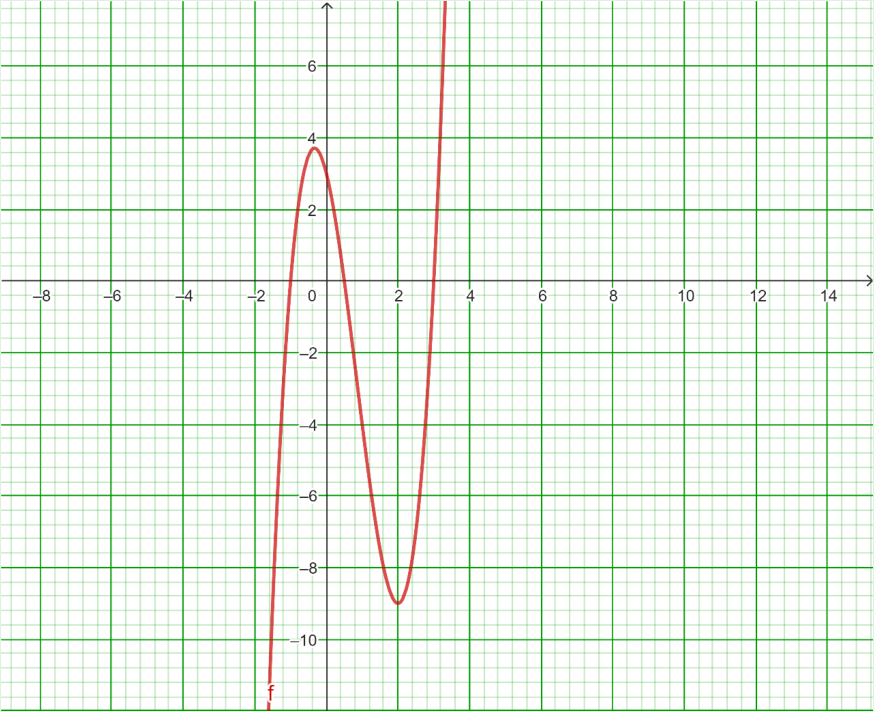
\includegraphics[width=0.7\linewidth]{figures/rq3-2.png}
\end{center}

\item Carefully, study the graph above which represents a polynomial function
f(x).
\begin{enumerate}
  \item[a.] State the zeros
  \item[b.] Find the factors
  \item[c.] State the interval on the curve.
  \item[d.] Find the polynomial function f(x)
\end{enumerate}

\item Sketch the following curves.
\begin{enumerate}
  \item[a.] $f(x) = x^3 + 2x^2 - 9x - 18$
  \item[b.] $f(x) = x^3 - 2x^2 - x + 2$
  \item[c.] $f(x) = x^3 + 3x^2 - 4x - 12$
  \item[d.] $f(x) = x^3 - 5x^2 - x + 5$
  \item[e.] $f(x) = \frac{1}{5}\left(x - 2\right)\left(x - 4\right)\left(x + 5\right)$
\end{enumerate}

\item Factorise:
\begin{enumerate}
  \item[a.] $x^3 + 5x^2 + 2x - 8$
  \item[b.] $2x^3 + 3x^2 - 17x - 30$
  \item[c.] $4x^3 - 4x^2 - 11x + 6$
  \item[d.] $6x^3 + 13x^2 - 4$
  \item[e.] $3x^3 + 16x^2 - 13x - 6$
\end{enumerate}

\item Find the zeros of the following:
\begin{enumerate}
  \item[a.] $x^3 + 4x^2 + x - 6$
  \item[b.] $2x^3 + 7x^2 - 14x + 5$
  \item[c.] $2x^3 + x^2 - 5x + 2$
  \item[d.] $4x^3 - 8x^2 - 9x + 18$
  \item[e.] $4x^3 - 4x^2 - x + 1$
  \item[f.] $4x^3 - 12x^2 + 11x - 3$
\end{enumerate}

\item Find the roots of:
\begin{enumerate}
  \item[a.] $x^3 + 6x$
  \item[b.] $2x^4 + 17x^2 + 35$
  \item[c.] $x^4 - 14x^2 + 36$
  \item[d.] $x^4 - 1$
  \item[e.] $x^3 + 27x$
\end{enumerate}
\begin{center}
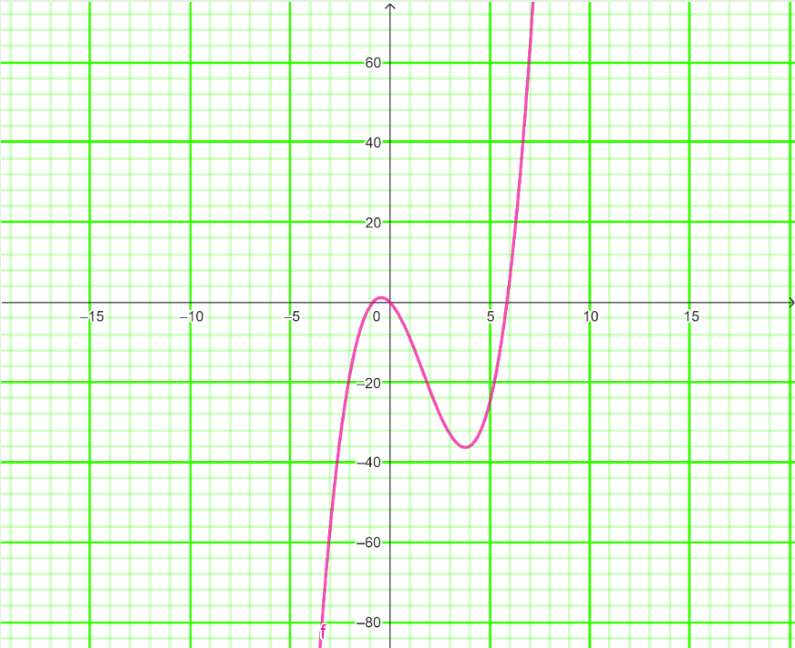
\includegraphics[width=0.65\linewidth]{figures/rq3-7.png}
\end{center}

\item Find the polynomial function f(x) as represented by the curve above.

\item $Q(x) = 10x^3 + ax^2 - 10x + b$, where $a$ and $b$ are integers, is divisible
by $(2x + 1)$. When $Q(x)$ is divided by $x + 1$, the remainder is -2.
\begin{enumerate}
  \item[a.] Find the values of a and of b
  \item[b.] find the expression for $Q(x)$ as a product of the three linear factors
\end{enumerate}

\item Given that $x_1 = 1 + \sqrt{2}\,i$ and $x_2 = 2 + 3i$ are roots of a polynomial
function $P(x)$, determine the $P(x) = 0$

\item Applying Descartes' Rule of Signs, identify the potential number of
positive and negative roots.
\begin{enumerate}
  \item[a.] $f(x) = 10x^6 - 5x^5 + 3x^4 - 6x^3 + 24x^2 - 38x$
  \item[b.] $f(x) = 19x^5 + 6x^4 + 17x^3 + 18x^2 - 38x - 70$
  \item[c.] $f(x) = x^6 - 729$
  \item[d.] $f(x) = 12x^6 + 13x^3 + 1$
  \item[e.] $f(x) = 8x^8 - 13x^4 + 100$
\end{enumerate}

\item Write down the equation having only the following roots.
\begin{enumerate}
  \item[a.] -5 , -1, 3
  \item[b.] $3, -\frac{1}{5}, -\frac{1}{3}$
  \item[c.] 2, -2, $2 + \sqrt{3}$, $2 - \sqrt{3}$
  \item[d.] 0, 1 $+$ 4i, 1- 4i
\end{enumerate}

\item Find the four roots of $y^4 + 3x^2 + 2$
\booknote[S3-16]{the polynomial mixes $y$ and $x$; the answer key treats it as
$y^4 + 3y^2 + 2$.}

\item Study the graph below and use it to answer the following questions:
\begin{enumerate}
  \item[a.] state the factors
  \item[b.] find the polynomial function
  \item[c.] how many turning points
  \item[d.] what is the relationship between the degree of the function and the
  number of turning points
\end{enumerate}
\begin{center}
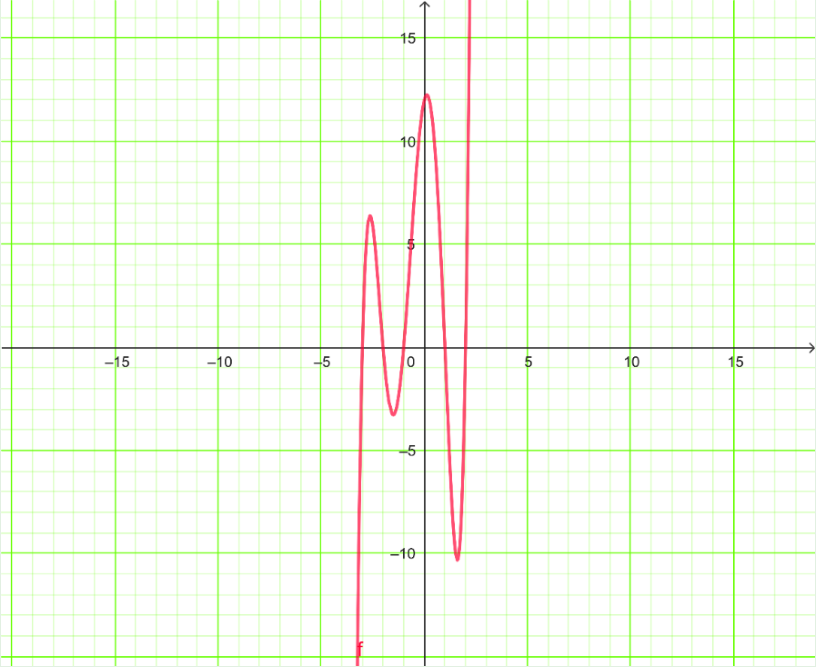
\includegraphics[width=0.65\linewidth]{figures/rq3-13.png}
\end{center}

\item A new bakery in Accra specialises in creating various types of bread. The
bakery wants the volume of a small rectangular loaf of bread to be 4 800
cm$^3$. The loaf is to be shaped like a rectangular solid. The length of the
loaf is to be 4cm longer than the width. The height of the loaf is one-half
of the width. Determine the dimensions of the loaf.
\end{enumerate}


\clearpage
\section*{Answers to Review Questions}
% Answers to the Section 3 Review Questions, book pp. 453-456 (PDF pp. 454-457).
% The answer key's own numbering, which matches the 14 printed questions.
\begin{enumerate}
\item
\begin{enumerate}
  \item[a.] $x = 3, -\frac{1}{3}, -\frac{1}{2}$
  \item[b.] $x = 1, -\frac{2}{5}, -1$
\end{enumerate}
\item
\begin{enumerate}
  \item[a.] the zeros are -1, 0.5. and 3
  \item[b.] the factors are $(x + 1)\,(2x\text{-}1)\,(x\text{-}3)$
  \item[c.] --1 $>$ x, --1 $<$ x $<$ 0.5, 0.5 $<$ x $<$ 3, x $>$ 3
  \item[d.] $f(x) = 2x^3 - 5x^2 - 4x + 3$
\end{enumerate}
\item
\begin{enumerate}
  \item[a.] \mbox{}\par\nopagebreak
  \begin{center}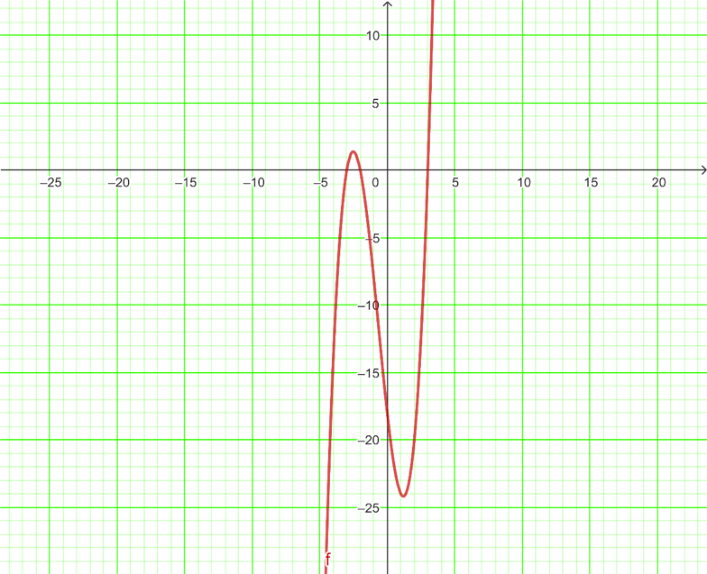
\includegraphics[width=0.55\linewidth]{figures/ans3-3a.png}\end{center}
  \item[b.] \mbox{}\par\nopagebreak
  \begin{center}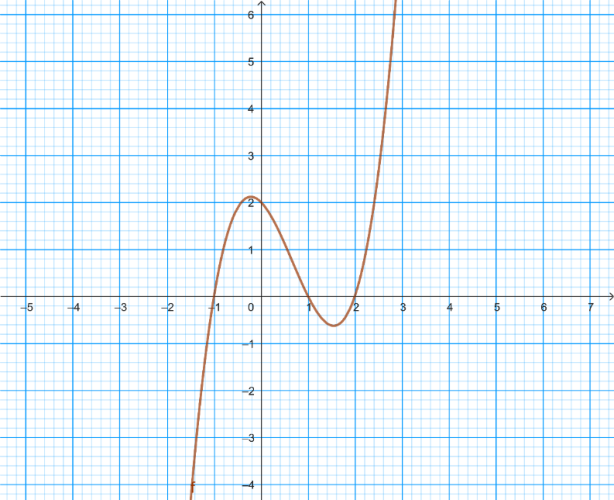
\includegraphics[width=0.55\linewidth]{figures/ans3-3b.png}\end{center}
  \item[c.] \mbox{}\par\nopagebreak
  \begin{center}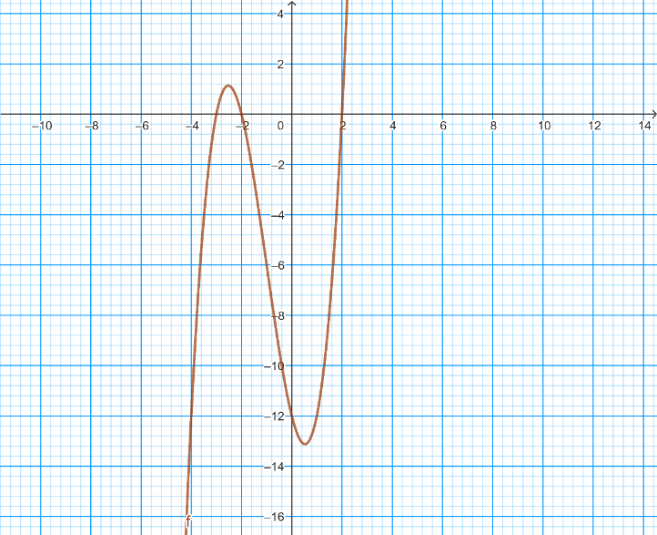
\includegraphics[width=0.55\linewidth]{figures/ans3-3c.png}\end{center}
  \item[d.] \mbox{}\par\nopagebreak
  \begin{center}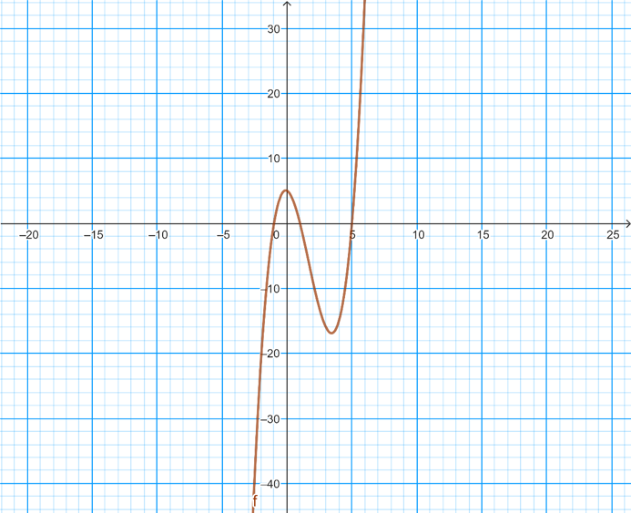
\includegraphics[width=0.55\linewidth]{figures/ans3-3d.png}\end{center}
  \item[e.] \mbox{}\par\nopagebreak
  \begin{center}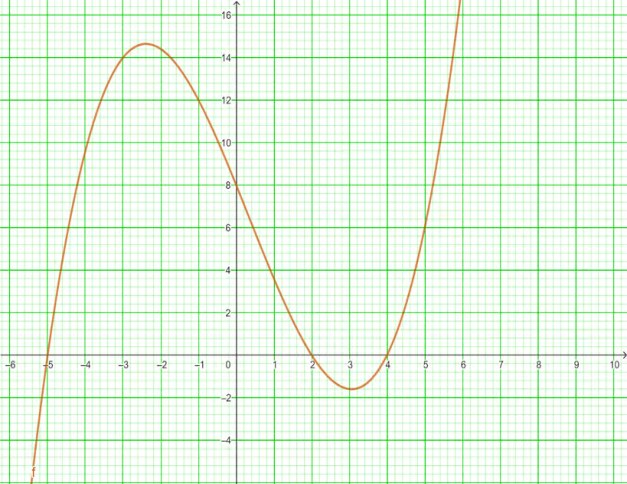
\includegraphics[width=0.55\linewidth]{figures/ans3-3e.jpg}\end{center}
\end{enumerate}
\item
\begin{enumerate}
  \item[a.] $(x - 1)(x + 2)(x + 4)$
  \item[b.] $(x + 2)(2x + 5)(x - 3)$
  \item[c.] $(x - 2)(2x -\ )(2x)$
  \booknote[S3-17]{the answer is garbled; $4x^3 - 4x^2 - 11x + 6 = (x - 2)(2x + 3)(2x - 1)$.}
  \item[d.] $(x + 2)(3x + 2)(2x - 1)$
  \item[e.] $(x - 1)(3x + 1)(x + 6)$
\end{enumerate}
\item
\begin{enumerate}
  \item[a.] $x = 1, -3, -2$
  \item[b.] $x = -5, 1, 0.5$
  \item[c.] $x = -2, 1, 0.5$
  \item[d.] $x = -1.5, 1.5, 2$
  \item[e.] $x = -0.5, 1, 0.5$
  \item[f.] $x = 1, 0.5, 1.5$
\end{enumerate}
\item
\begin{enumerate}
  \item[a.] $0, i\sqrt{6}, -i\sqrt{6}$
  \item[b.] $i\sqrt{\frac{7}{2}}, -i\sqrt{\frac{7}{2}}, -\sqrt{5}, \sqrt{5}$
  \booknote[S3-18]{$2x^4 + 17x^2 + 35 = (2x^2 + 7)(x^2 + 5)$, so the last two roots
  are $-i\sqrt{5}$ and $i\sqrt{5}$.}
  \item[c.] $-\sqrt{7 + \sqrt{13}},\ ,\ \sqrt{7 + \sqrt{13}}, -\sqrt{7 - \sqrt{13}},
  \sqrt{7 - \sqrt{13}}$
  \item[d.] $1, -1, i, -i$
  \item[e.] $0, 3i\sqrt{3}, -3i\sqrt{3}$
\end{enumerate}
\item $f(x) = x^3 - 5x^2 - 6x$
\item
\begin{enumerate}
  \item[a.] a $=$ 11, b $=$ 6
  \item[b.] $(2x + 1)(x + 2)(x + 3)$
\end{enumerate}
\booknote[S3-19]{this answer does not fit the question: $(2x + 1)(x + 2)(x + 3)
= 2x^3 + 11x^2 + 17x + 6$, whose leading coefficient is 2, not 10, and with
$a = 11$, $b = 6$ the printed $Q(x)$ gives $Q(-\frac{1}{2}) = 12.5$ and
$Q(-1) = 17$. The conditions as printed have no integer solution.}
\item $f(x) = x^4 - 6x^3 + 24x^2 - 38x + 29$
\booknote[S3-20]{$(x^2 - 2x + 3)(x^2 - 4x + 13) = x^4 - 6x^3 + 24x^2 - 38x + 39$;
the constant term should be 39.}
\item
\begin{enumerate}
  \item[a.] Positive zeros\textbf{:} 5, 3, or 1, Negative zeros\textbf{:} 0
  \item[b.] Possible Positive Zeros\textbf{:} 1, Possible Negative Zeros\textbf{:} 4, 2, or 0
  \item[c.] Possible Positive Zeros\textbf{:} 1, Possible Negative Zeros\textbf{:} 1
  \item[d.] Possible Positive Zeros\textbf{:} 0, Possible Negative Zeros\textbf{:} 2 or 0
  \item[e.] Possible Positive Zeros\textbf{:} 2 or 0, Possible Negative Zeros\textbf{:} 2 or 0
\end{enumerate}
\item
\begin{enumerate}
  \item[a.] $x^3 + 3x^2 - 13x - 15$
  \item[b.] $15x^3 - 37x^2 - 23x - 3$
  \item[c.] $x^4 - 8x^2 + 16$
  \booknote[S3-21]{$x^4 - 8x^2 + 16 = (x^2 - 4)^2$ has roots $\pm 2$ only; the
  equation with roots $2, -2, 2 \pm \sqrt{3}$ is $(x^2 - 4)(x^2 - 4x + 1) =
  x^4 - 4x^3 - 3x^2 + 16x - 4$.}
  \item[d.] $x^3 - 2x^2 + 17x$
\end{enumerate}
\item $i, -i, i\sqrt{2}, -i\sqrt{2}$
\item
\begin{enumerate}
  \item[a.] $(x + 1)(x + 2)(x + 3)(x - 1)(x - 2)$
  \item[b.] $x^5 + 3x^4 - 5x^3 - 15x^2 + 4x + 12$
  \item[c.] 4 turning points
  \item[d.] degree reduced by 1 gives the maximum number of turning points
\end{enumerate}
\item Width $=$ 20 cm, Length $=$ 24cm and Height $=$ 10 cm.
\end{enumerate}


\end{document}
